\chapter{Results} \label{ch:result} During the training sessions, we have recorded five static gestures in 4 different positions in front of the robot. NAO is equipped with Asus Xtion and set in "Stand" posture. Head pitch of NAO is set to -18 degrees to look at the upper body of the user 1800 mm away from the sensor. First 3 positions of training are recorded at 1800 mm distance from the sensor in z axis and + /- 800 mm in x axis. Last training position is recorded at 2200 mm distance. Therefore, training data is recorded for 80 seconds of each gesture.

In this chapter, we present the results of real time hand gesture recognition for Human-robot interaction based on skeletal points tracking using depth camera. Training data for 5 classes with 11918 samples of 6 dimensional vector are trained with Adaptive Naive Bayes Classifier (ANBC). Min-Max scaling and Null Rejection with coefficient of 2.0 are enabled. Following sections illustrates the results of end-to-end interaction with robot using five gestures named as Walk, Turn Right, Turn Left, Move Right, Move Left gestures which are mapped to class labels 1,2,3,4,5 respectively.

\clearpage 
\section{Gesture-To-Motion} 
\subsection{Walk} Figure \ref{res:gm:walk} shows that NAO is looking at the user to detect any possible gestures. When it recognized Walk gesture, Command module commands the robot to walk in forward direction for five seconds, thereby, completing a Gesture-To-Motion translation.

\begin{figure}
	[h] 
	\begin{minipage}
		{1 
		\textwidth} \centering 
		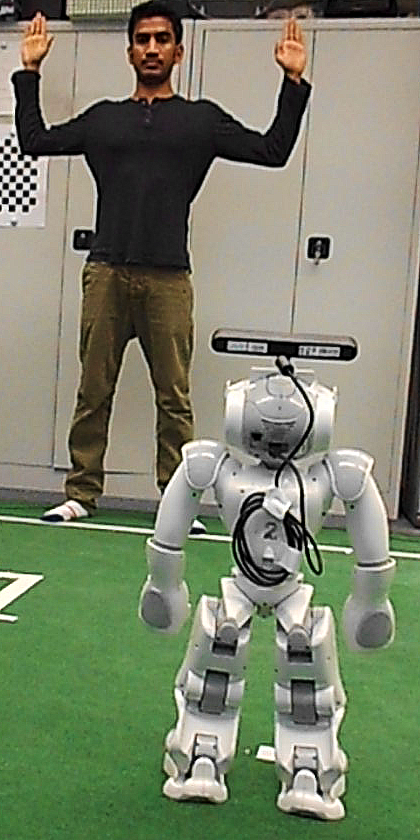
\includegraphics[height=75mm]{figures/result/res-ges-walk.png} \caption*{} 
	\end{minipage}
	\begin{minipage}
		{1 
		\textwidth} 
		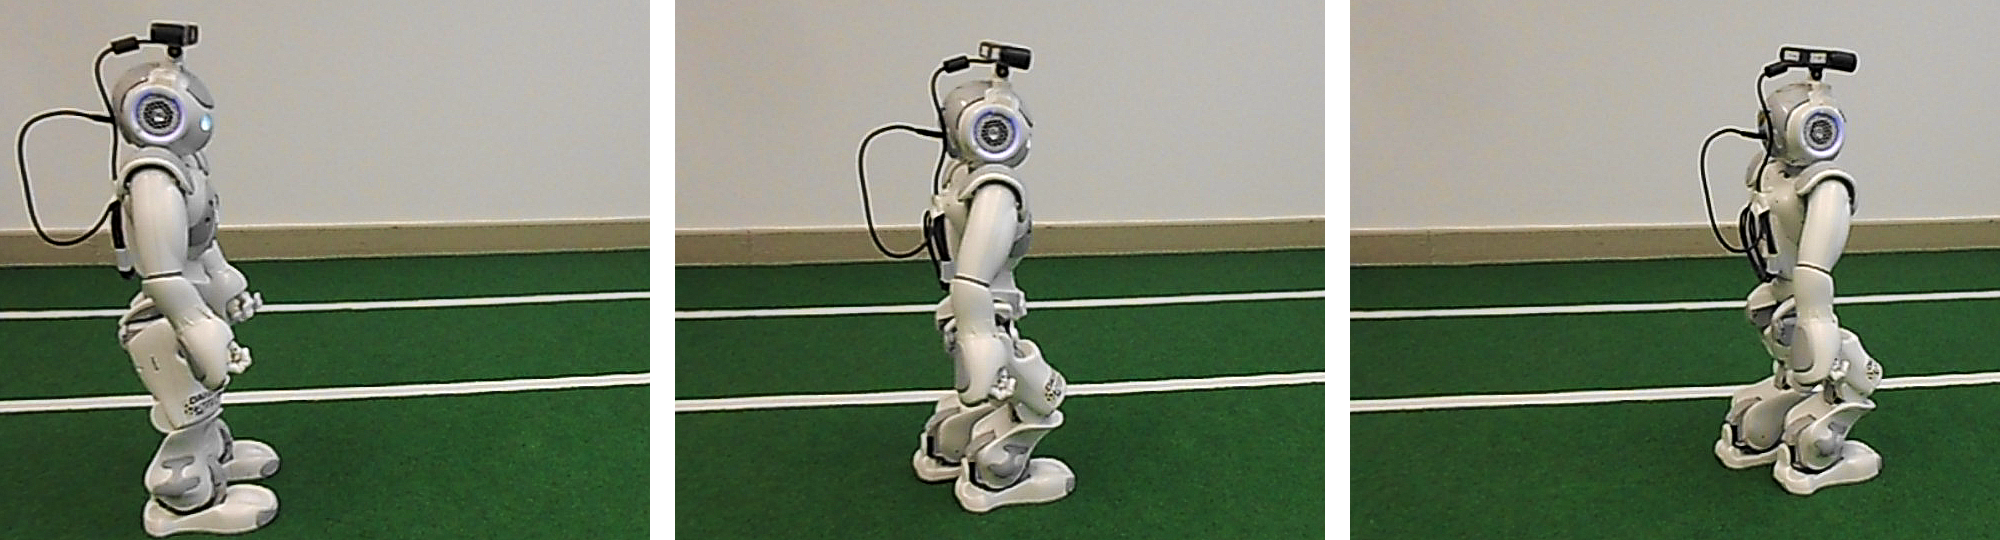
\includegraphics[height=42mm]{figures/result/nao-gm-walk.png} 
	\end{minipage}
\end{figure}


Graph \ref{res:pl:walk} shows the positions of left and right hand in x and y coordinates from the origin of the sensor. It is plotted using 60 input samples of Walk gesture. Figure \ref{res:cc:walk} shows the dashboard of Control Center that displays the prediction results. 

\clearpage 
\subsection{Turn Right} Figure \ref{res:gm:turn:right} shows that NAO received the input samples of left and right hand, and it recognized Turn Right gesture. The user commands NAO to turn at his right direction, thus, NAO turns at the mirrored direction (Left) for 5 seconds and stops to look for further gestures.

\begin{figure}
	[h] 
	\begin{minipage}
		{1 
		\textwidth} \centering 
		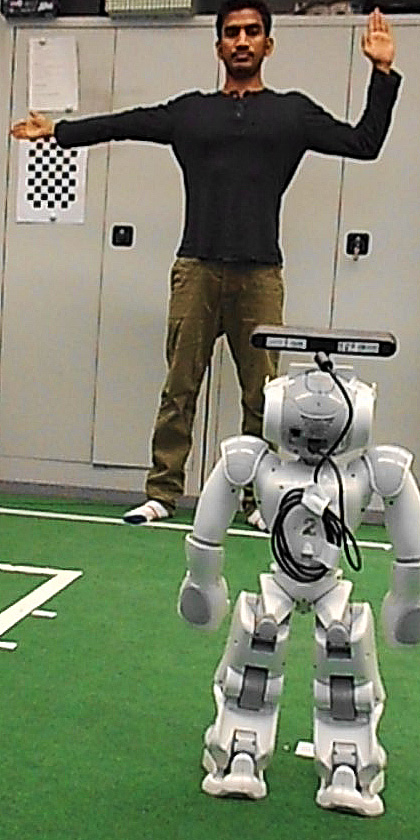
\includegraphics[height=95mm]{figures/result/usr-turn-right.jpg} \caption*{} 
	\end{minipage}
	\begin{minipage}
		{1 
		\textwidth} \hspace{-5 mm} 
		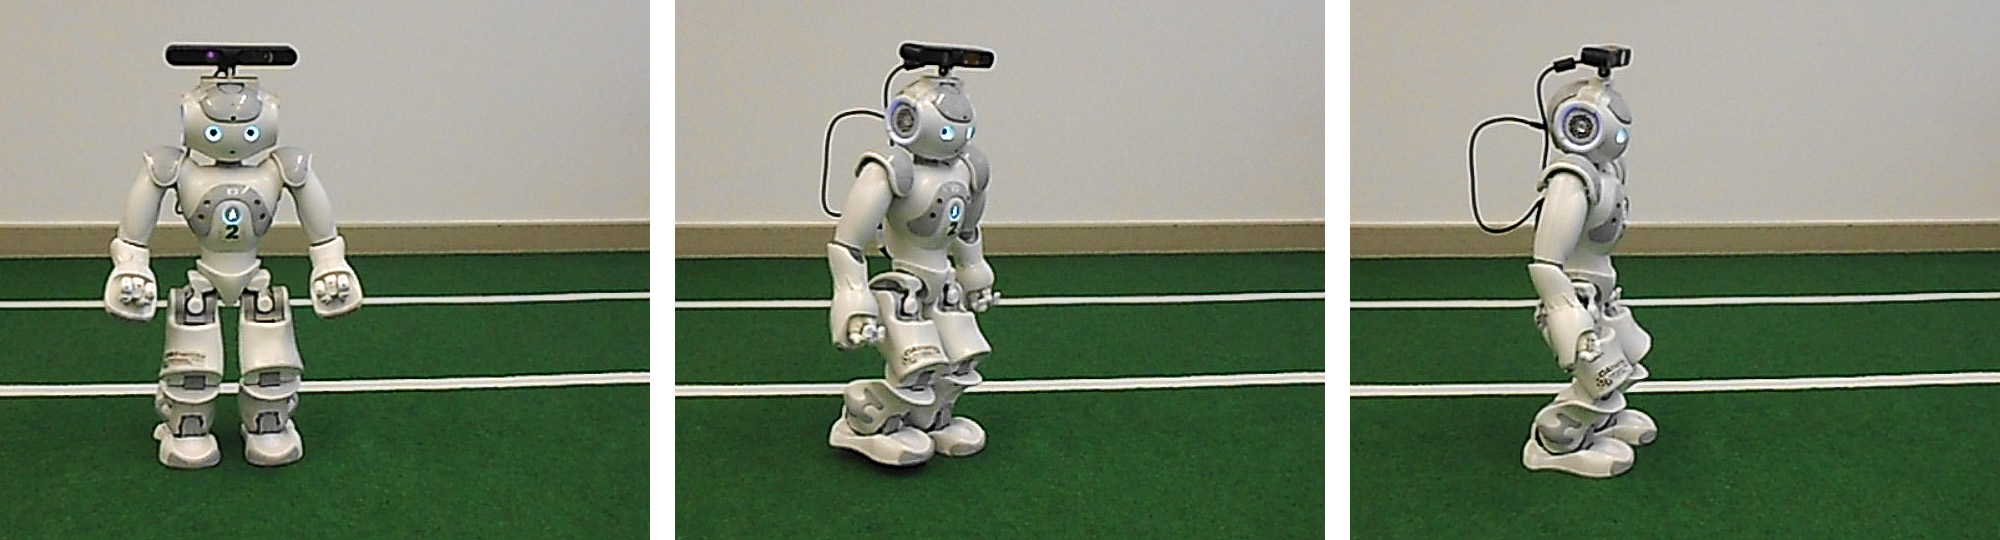
\includegraphics[width=160mm]{figures/result/nao-gm-turn-right.jpg} 
	\end{minipage}
	\caption{NAO recognizes Turn Right gesture and executes a predefined Gesture-To-Motion task.} \label{res:gm:turn:right} 
\end{figure}
\begin{figure}
	[h] \hspace{-15 mm} \centering 
	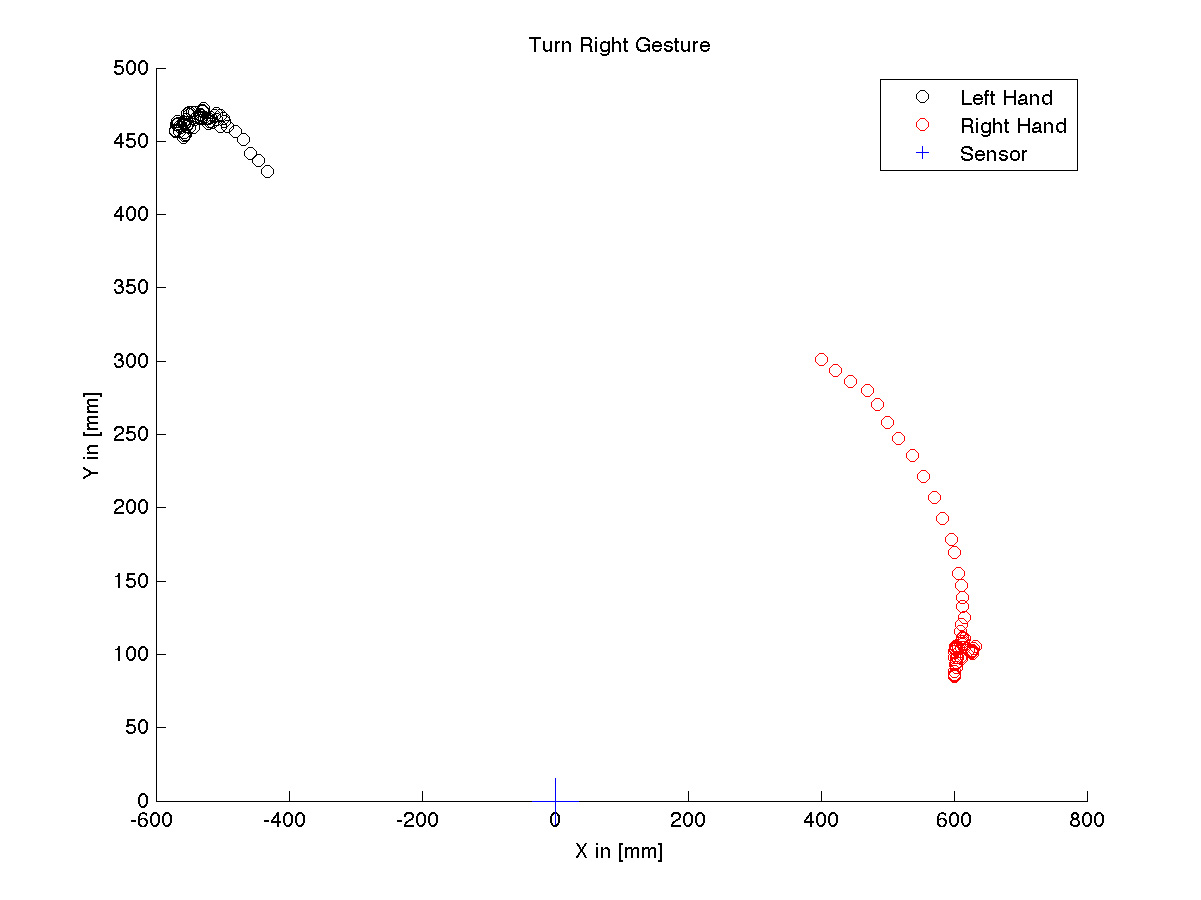
\includegraphics[width=155mm]{figures/result/test-turn-right.jpg} \caption{Our system is capable of real time prediction by processing 30 samples per second. However, the detected hand gesture is triggered only when it is gesticulated for 1 second because of the post-processing by Class Label Filter module. The graph shows 60 samples of correctly recognized Turn Right gesture. } \label{res:pl:turn:right} 
\end{figure}
\begin{figure}
	[h] \centering 
	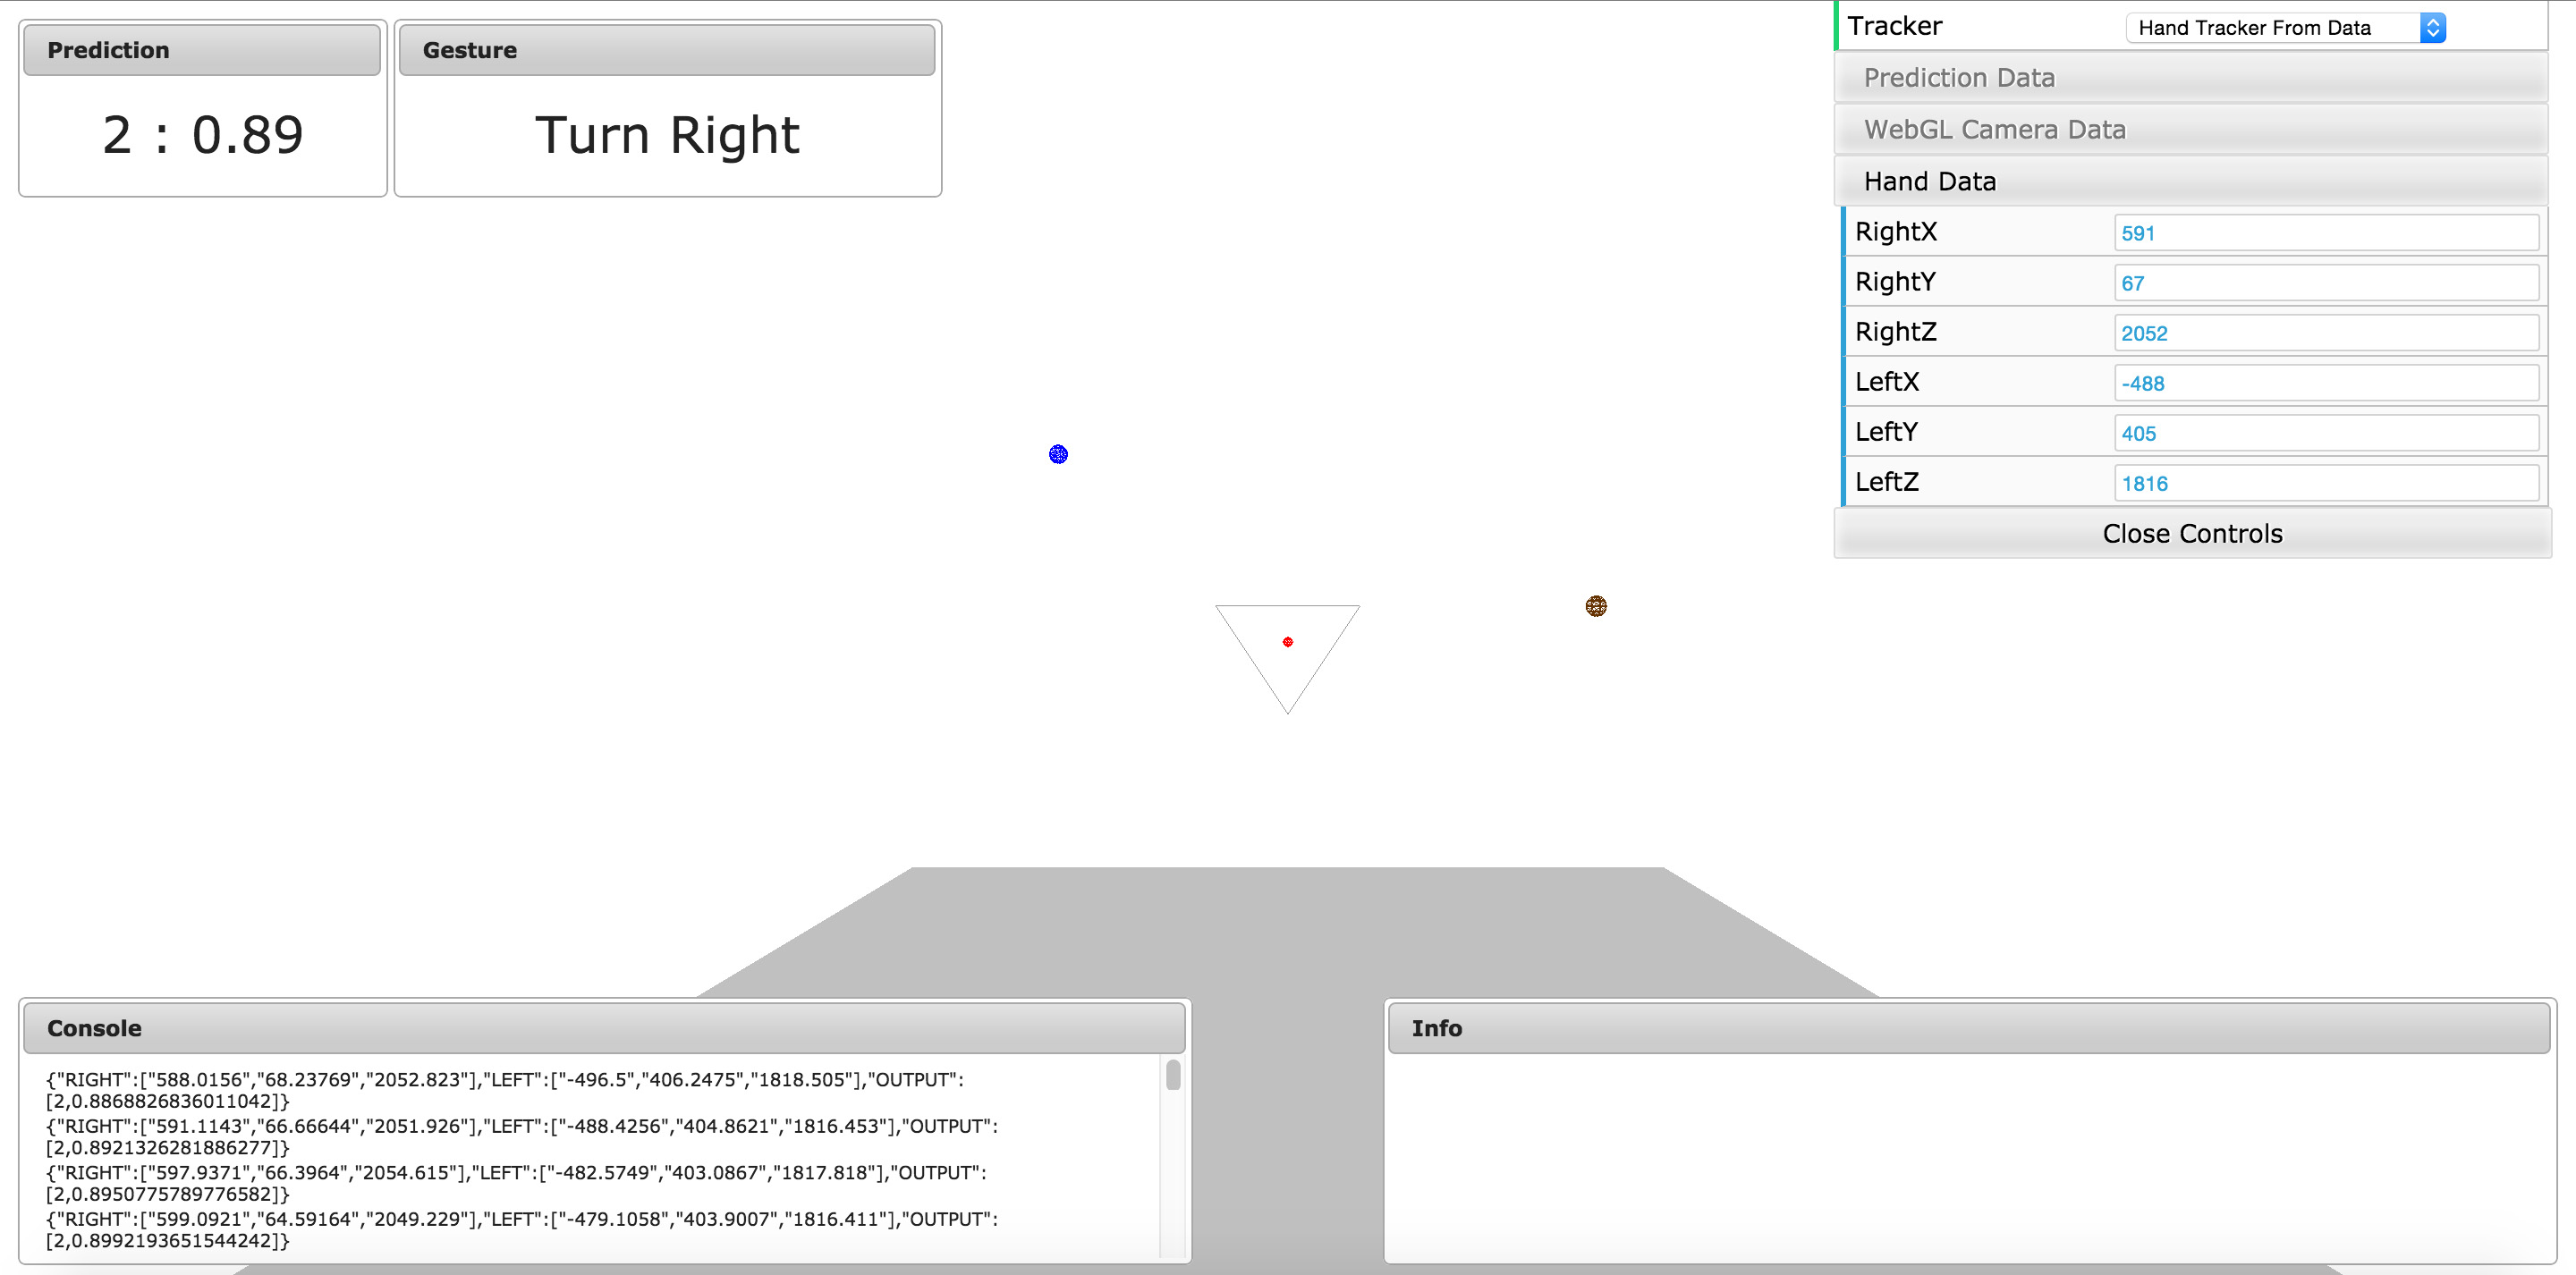
\includegraphics[height=70mm]{figures/result/cc-turn-right.jpg} \caption{Control Center displays the recognized Turn Right gesture in real time with the positions of left and right hand in 3 dimensional space.} \label{res:cc:turn:right} 
\end{figure}


Graph \ref{res:pl:turn:right} shows the positions of left and right hand in x and y coordinates from the origin of the sensor. It is plotted using 60 input samples of Turn Right gesture. Figure \ref{res:cc:turn:right} shows the dashboard of Control Center that displays the prediction results. 

\clearpage 
\subsection{Turn Left} Figure \ref{res:gm:turn:left} shows that NAO received the input samples of left and right hand, and it recognized Turn Left gesture. The user commands NAO to turn at his left direction, thus, NAO turns at the mirrored direction (Right) for 5 seconds and stops to look for further gestures.

\begin{figure}
	[h] 
	\begin{minipage}
		{1 
		\textwidth} \centering 
		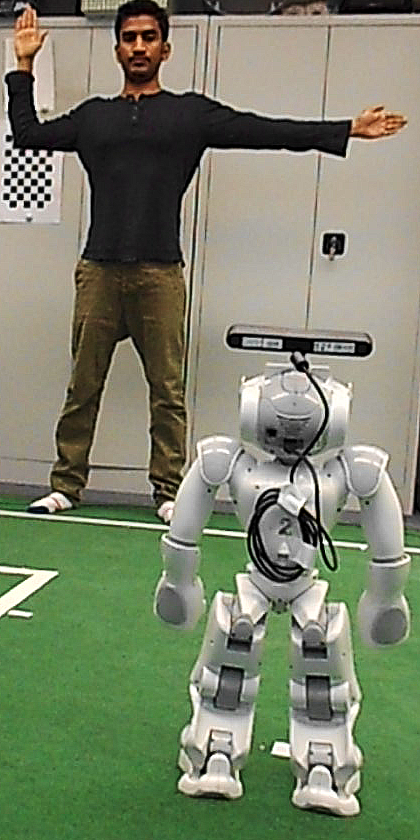
\includegraphics[height=75mm]{figures/result/res-ges-turn-left.png} \caption*{} 
	\end{minipage}
	\begin{minipage}
		{1 
		\textwidth} 
		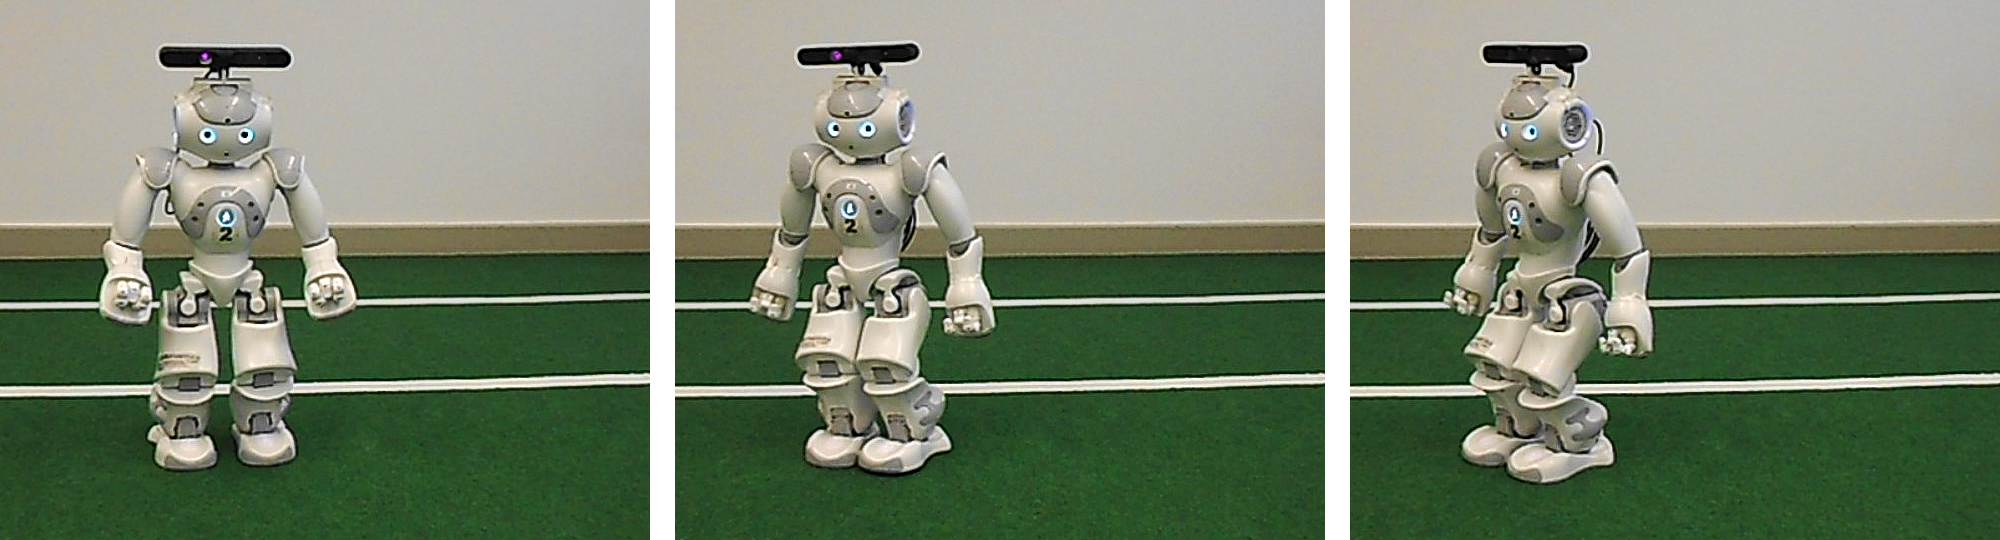
\includegraphics[height=42mm]{figures/result/nao-gm-turn-left.png} 
	\end{minipage}
\end{figure}


Graph \ref{res:pl:turn:left} shows the positions of left and right hand in x and y coordinates from the origin of the sensor. It is plotted using 60 input samples of Turn Left gesture. Figure \ref{res:cc:turn:left} shows the dashboard of Control Center that displays the prediction results. 

\clearpage 
\subsection{Move Right} Figure \ref{res:gm:move:right} shows that NAO recognizes Move Right gesture as soon as the user gesticulated it using both the tracked hands. Like other gestures, this is also perceived by NAO to move in the mirrored direction of the user. Hence, NAO turns left for 3 seconds and move in forward direction for 5 seconds.

\begin{figure}
	[h] 
	\begin{minipage}
		{0.3 
		\textwidth} 
		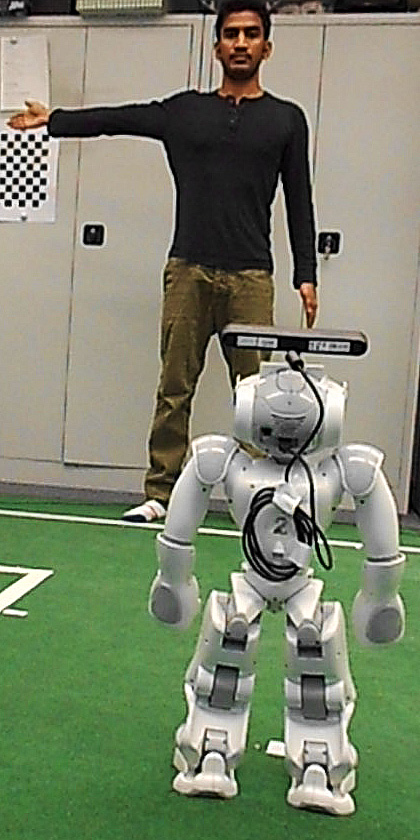
\includegraphics[height=80mm]{/result/usr-move-right.jpg} \caption*{(a)} 
	\end{minipage}
	\begin{minipage}
		{0.7
			\textwidth} 
		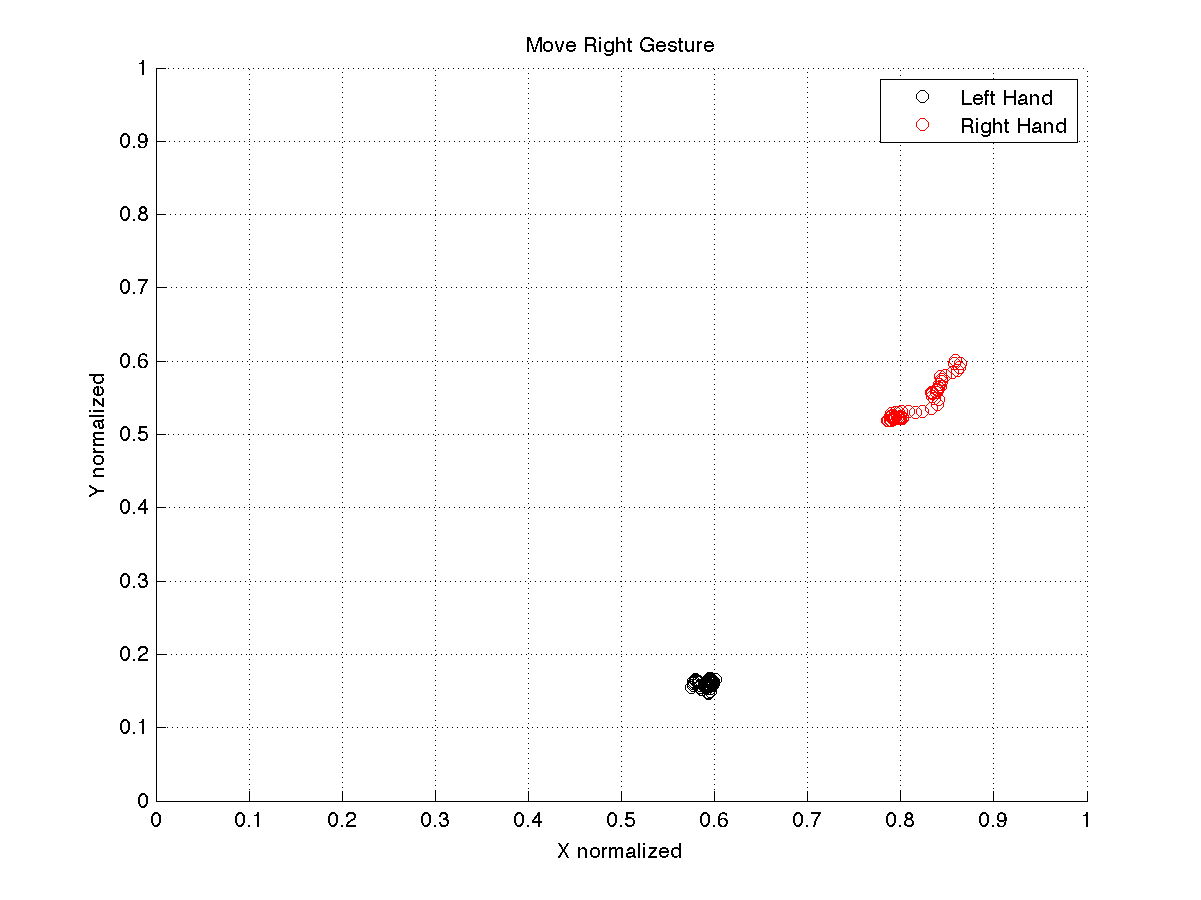
\includegraphics[width=110mm]{/result/test-move-right.png} \caption*{(b)} 
	\end{minipage}
	\begin{minipage}
		{0.3
		\textwidth}
		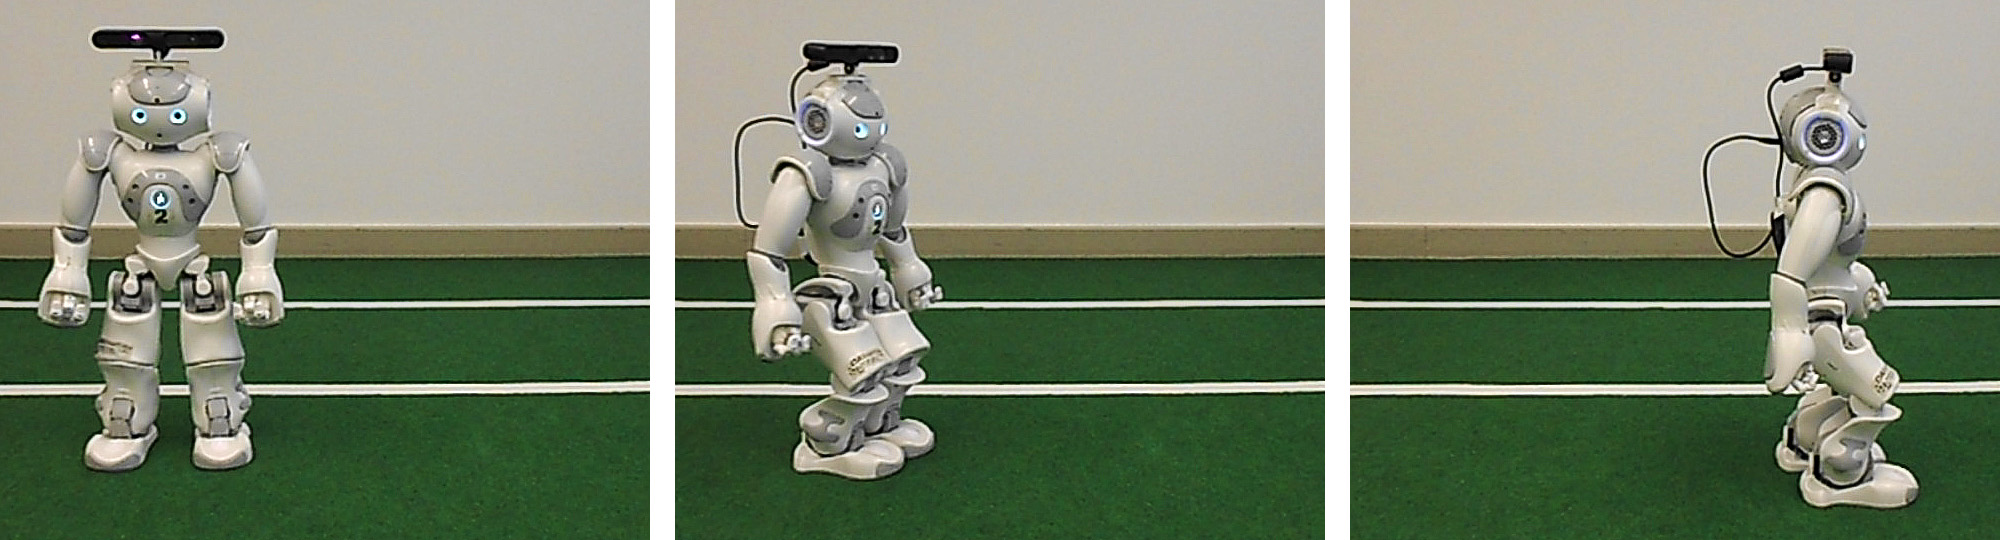
\includegraphics[height=100mm]{/result/nao-gm-move-right.jpg} \caption*{(d)} 
	\end{minipage}
	\begin{minipage}
		{0.7
			\textwidth}
		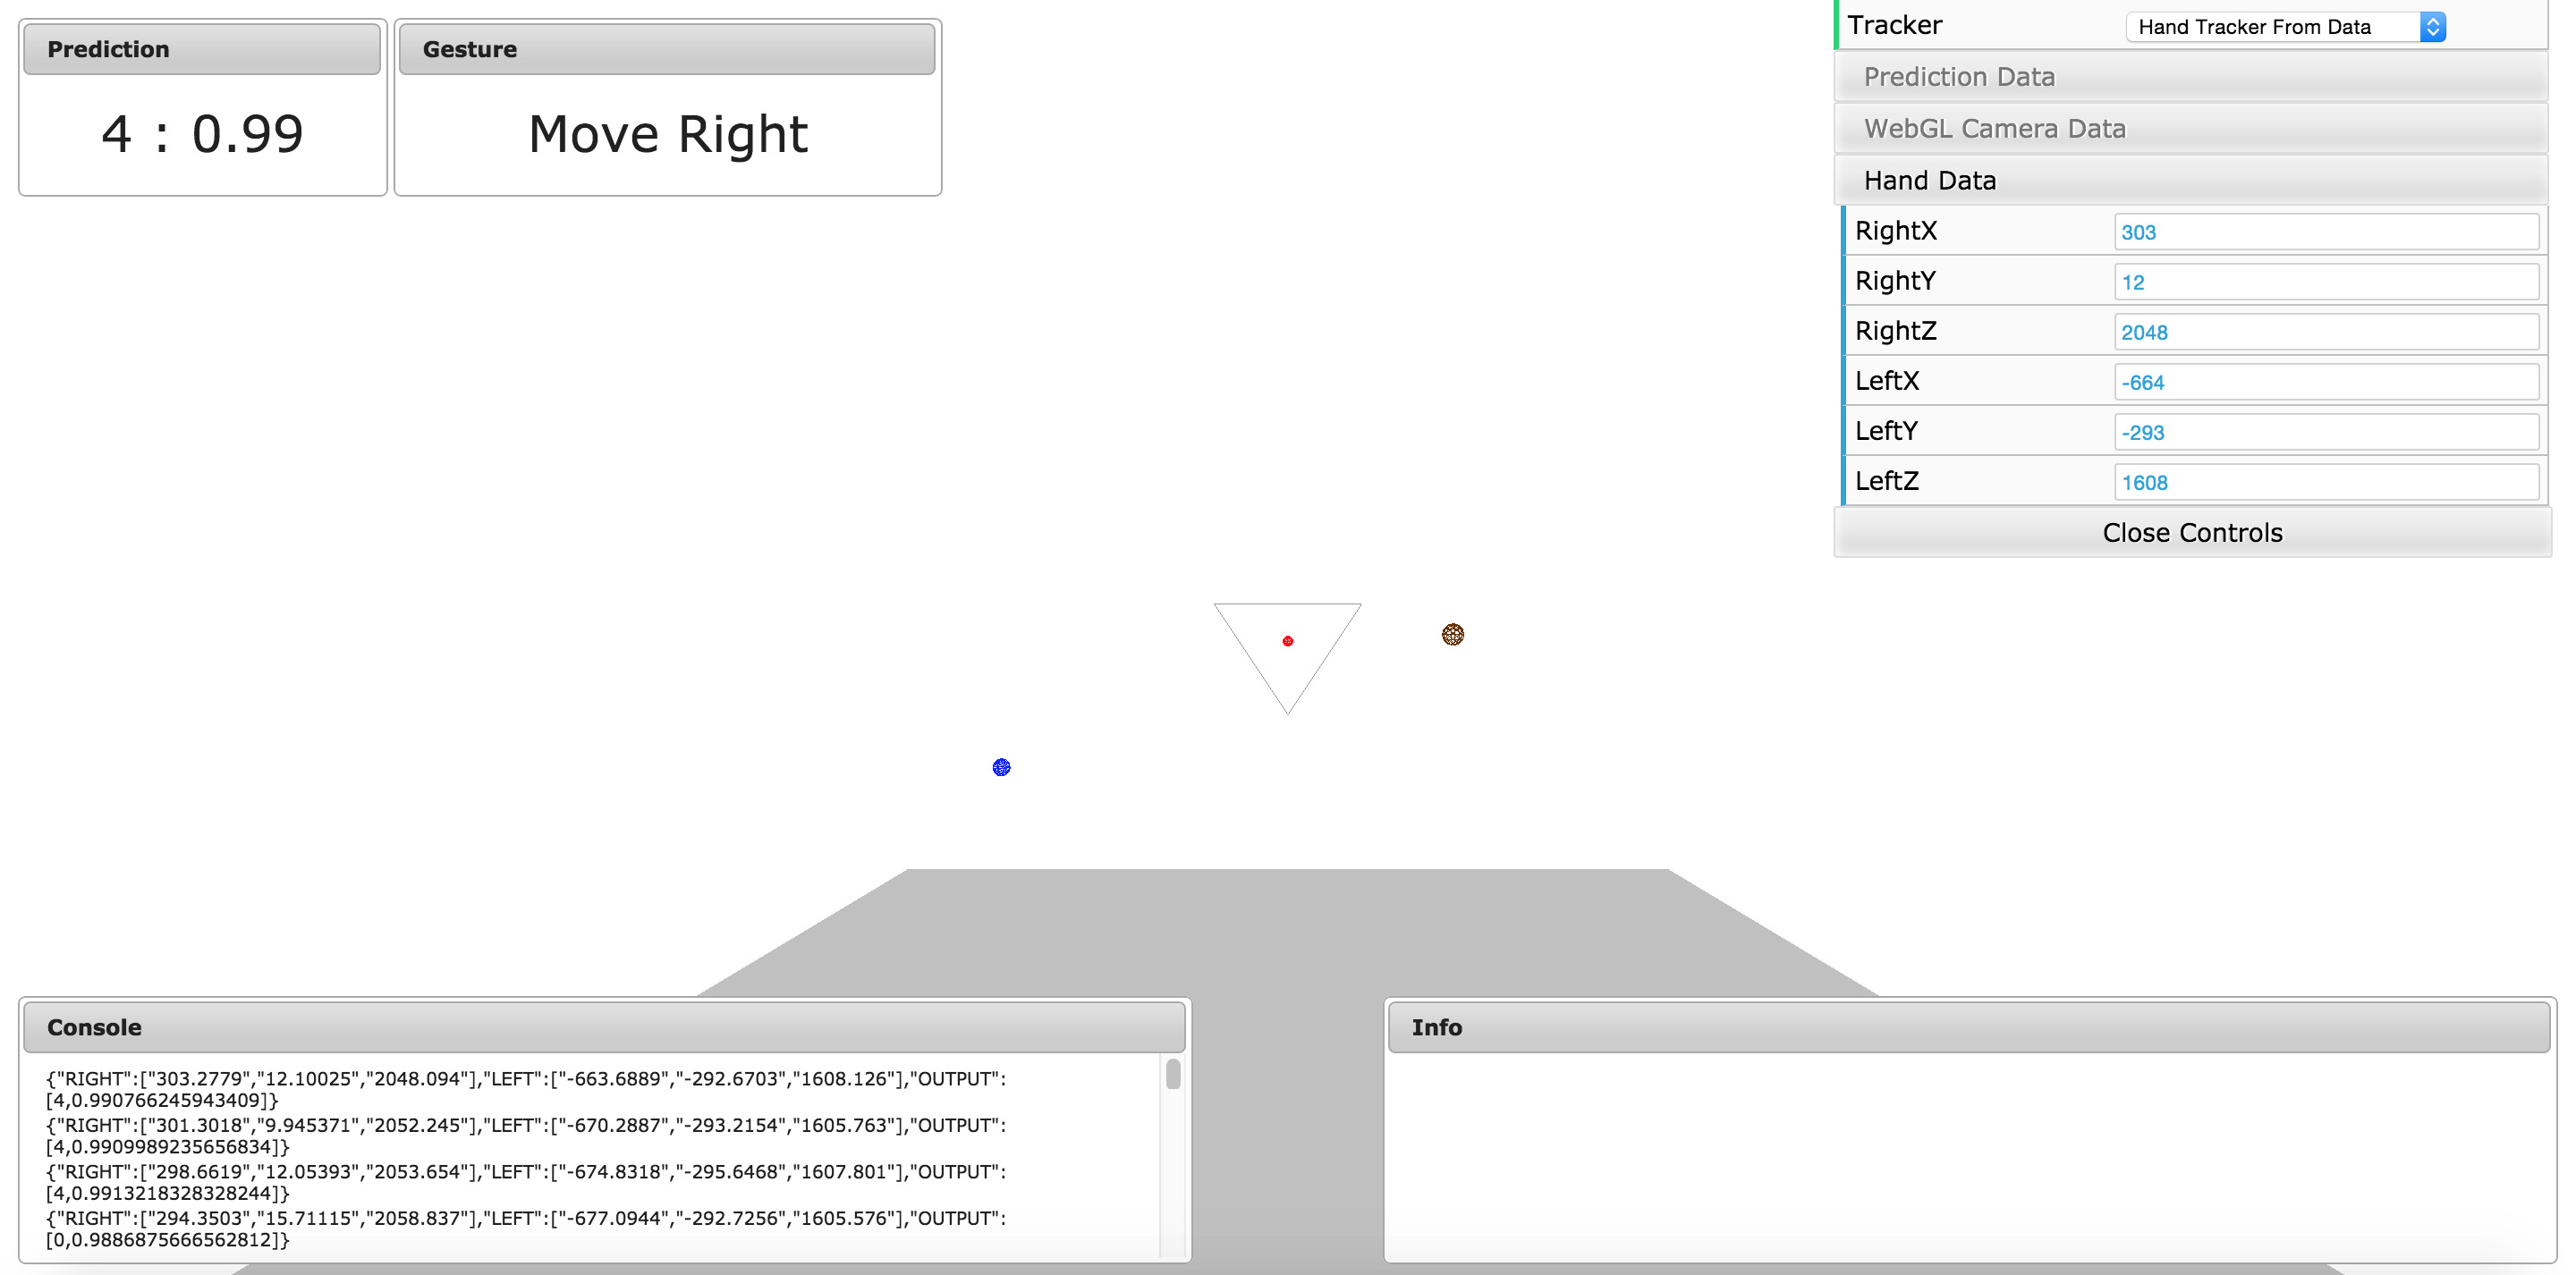
\includegraphics[width=100mm]{/result/cc-move-right.jpg}	\caption*{(c)} 
	\end{minipage}
	\caption{(a) User gesticulating Move Right gesture. (b) Normalized x,y positions of both hands. (c) CC dashboard shows the prediction results. (d) NAO executes Gesture-To-Motion Task.} \label{res:gm:move-right} 
\end{figure}

Graph \ref{res:pl:move:right} shows the positions of left and right hand in x and y coordinates from the origin of the sensor. It is plotted using 60 input samples of Move Right gesture. Figure \ref{res:cc:move:right} shows the dashboard of Control Center that displays the prediction results. 

\clearpage 
\subsection{Move Left} Figure \ref{res:gm:move:left} shows that NAO recognizes Move Left gesture as soon as the user gesticulated it using both the tracked hands. Like other gestures, this is also perceived by NAO to move in the mirrored direction of the user. Hence, NAO turns right for 3 seconds and move in forward direction for 5 seconds.

\begin{figure}
	[h] 
	\begin{minipage}
		{1 
		\textwidth} \centering 
		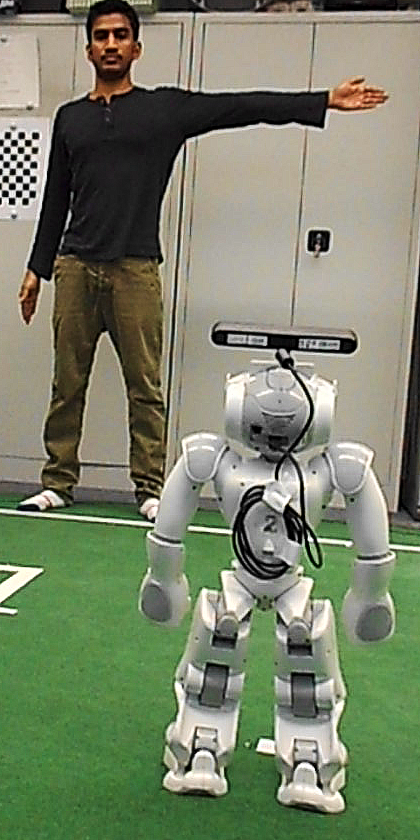
\includegraphics[height=75mm]{figures/result/res-ges-move-left.png} \caption*{} 
	\end{minipage}
	\begin{minipage}
		{1 
		\textwidth} 
		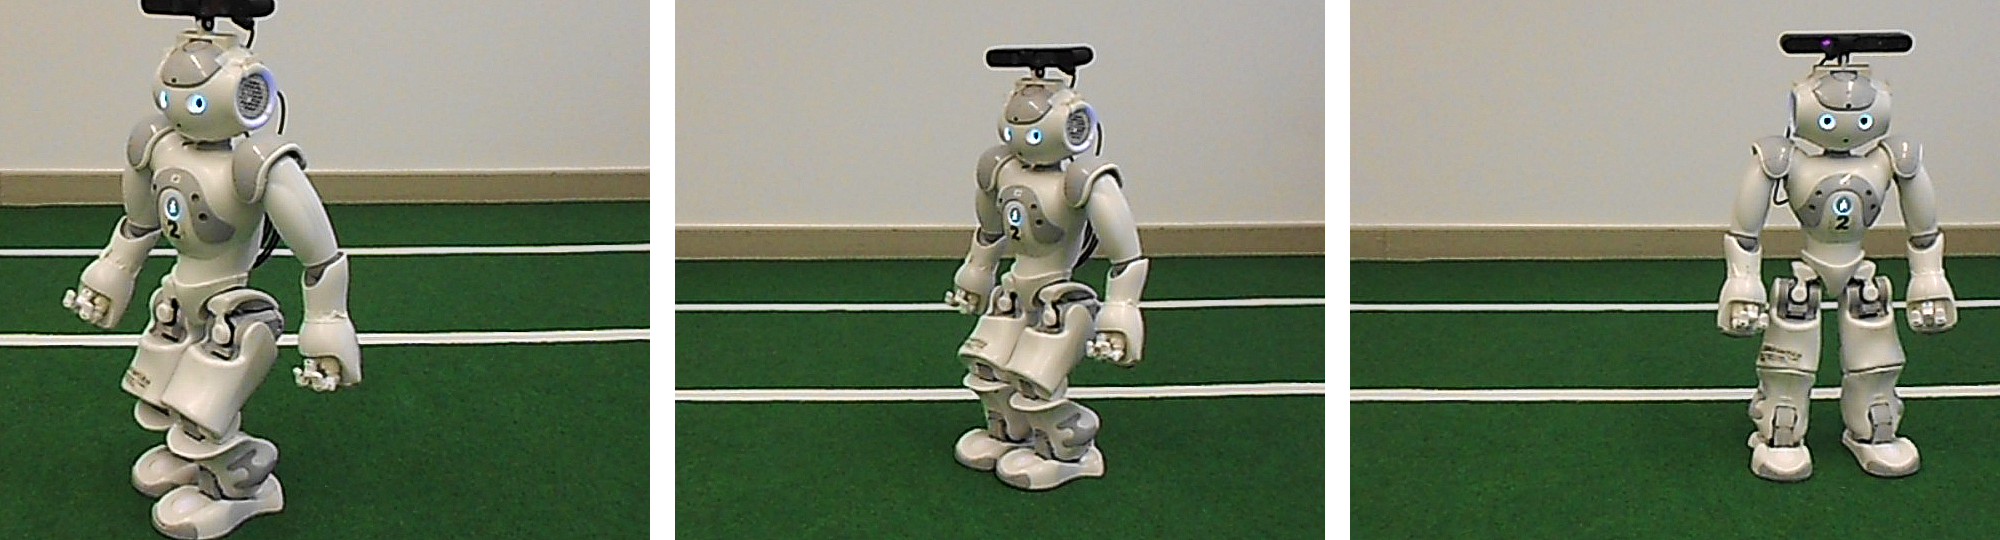
\includegraphics[height=42mm]{figures/result/nao-gm-move-left.png} 
	\end{minipage}
\end{figure}


Graph \ref{res:pl:move:left} shows the positions of left and right hand in x and y coordinates from the origin of the sensor. It is plotted using 60 input samples of Move Left gesture. Figure \ref{res:cc:move:left} shows the dashboard of Control Center that displays the prediction results. 

\clearpage

\section{Gesture-To-Gesture} Figure \ref{res:gg} shows how human hand gestures are translated to robotic hand gestures. When a gesture is detected, the Command module sets the predefined angles to the shoulder and elbow joints of both the hands of NAO to perform Gesture-To-Gesture translation. \begin{figure}
	[h]	 	
	\begin{minipage}
		{.3 
			\textwidth}  		
		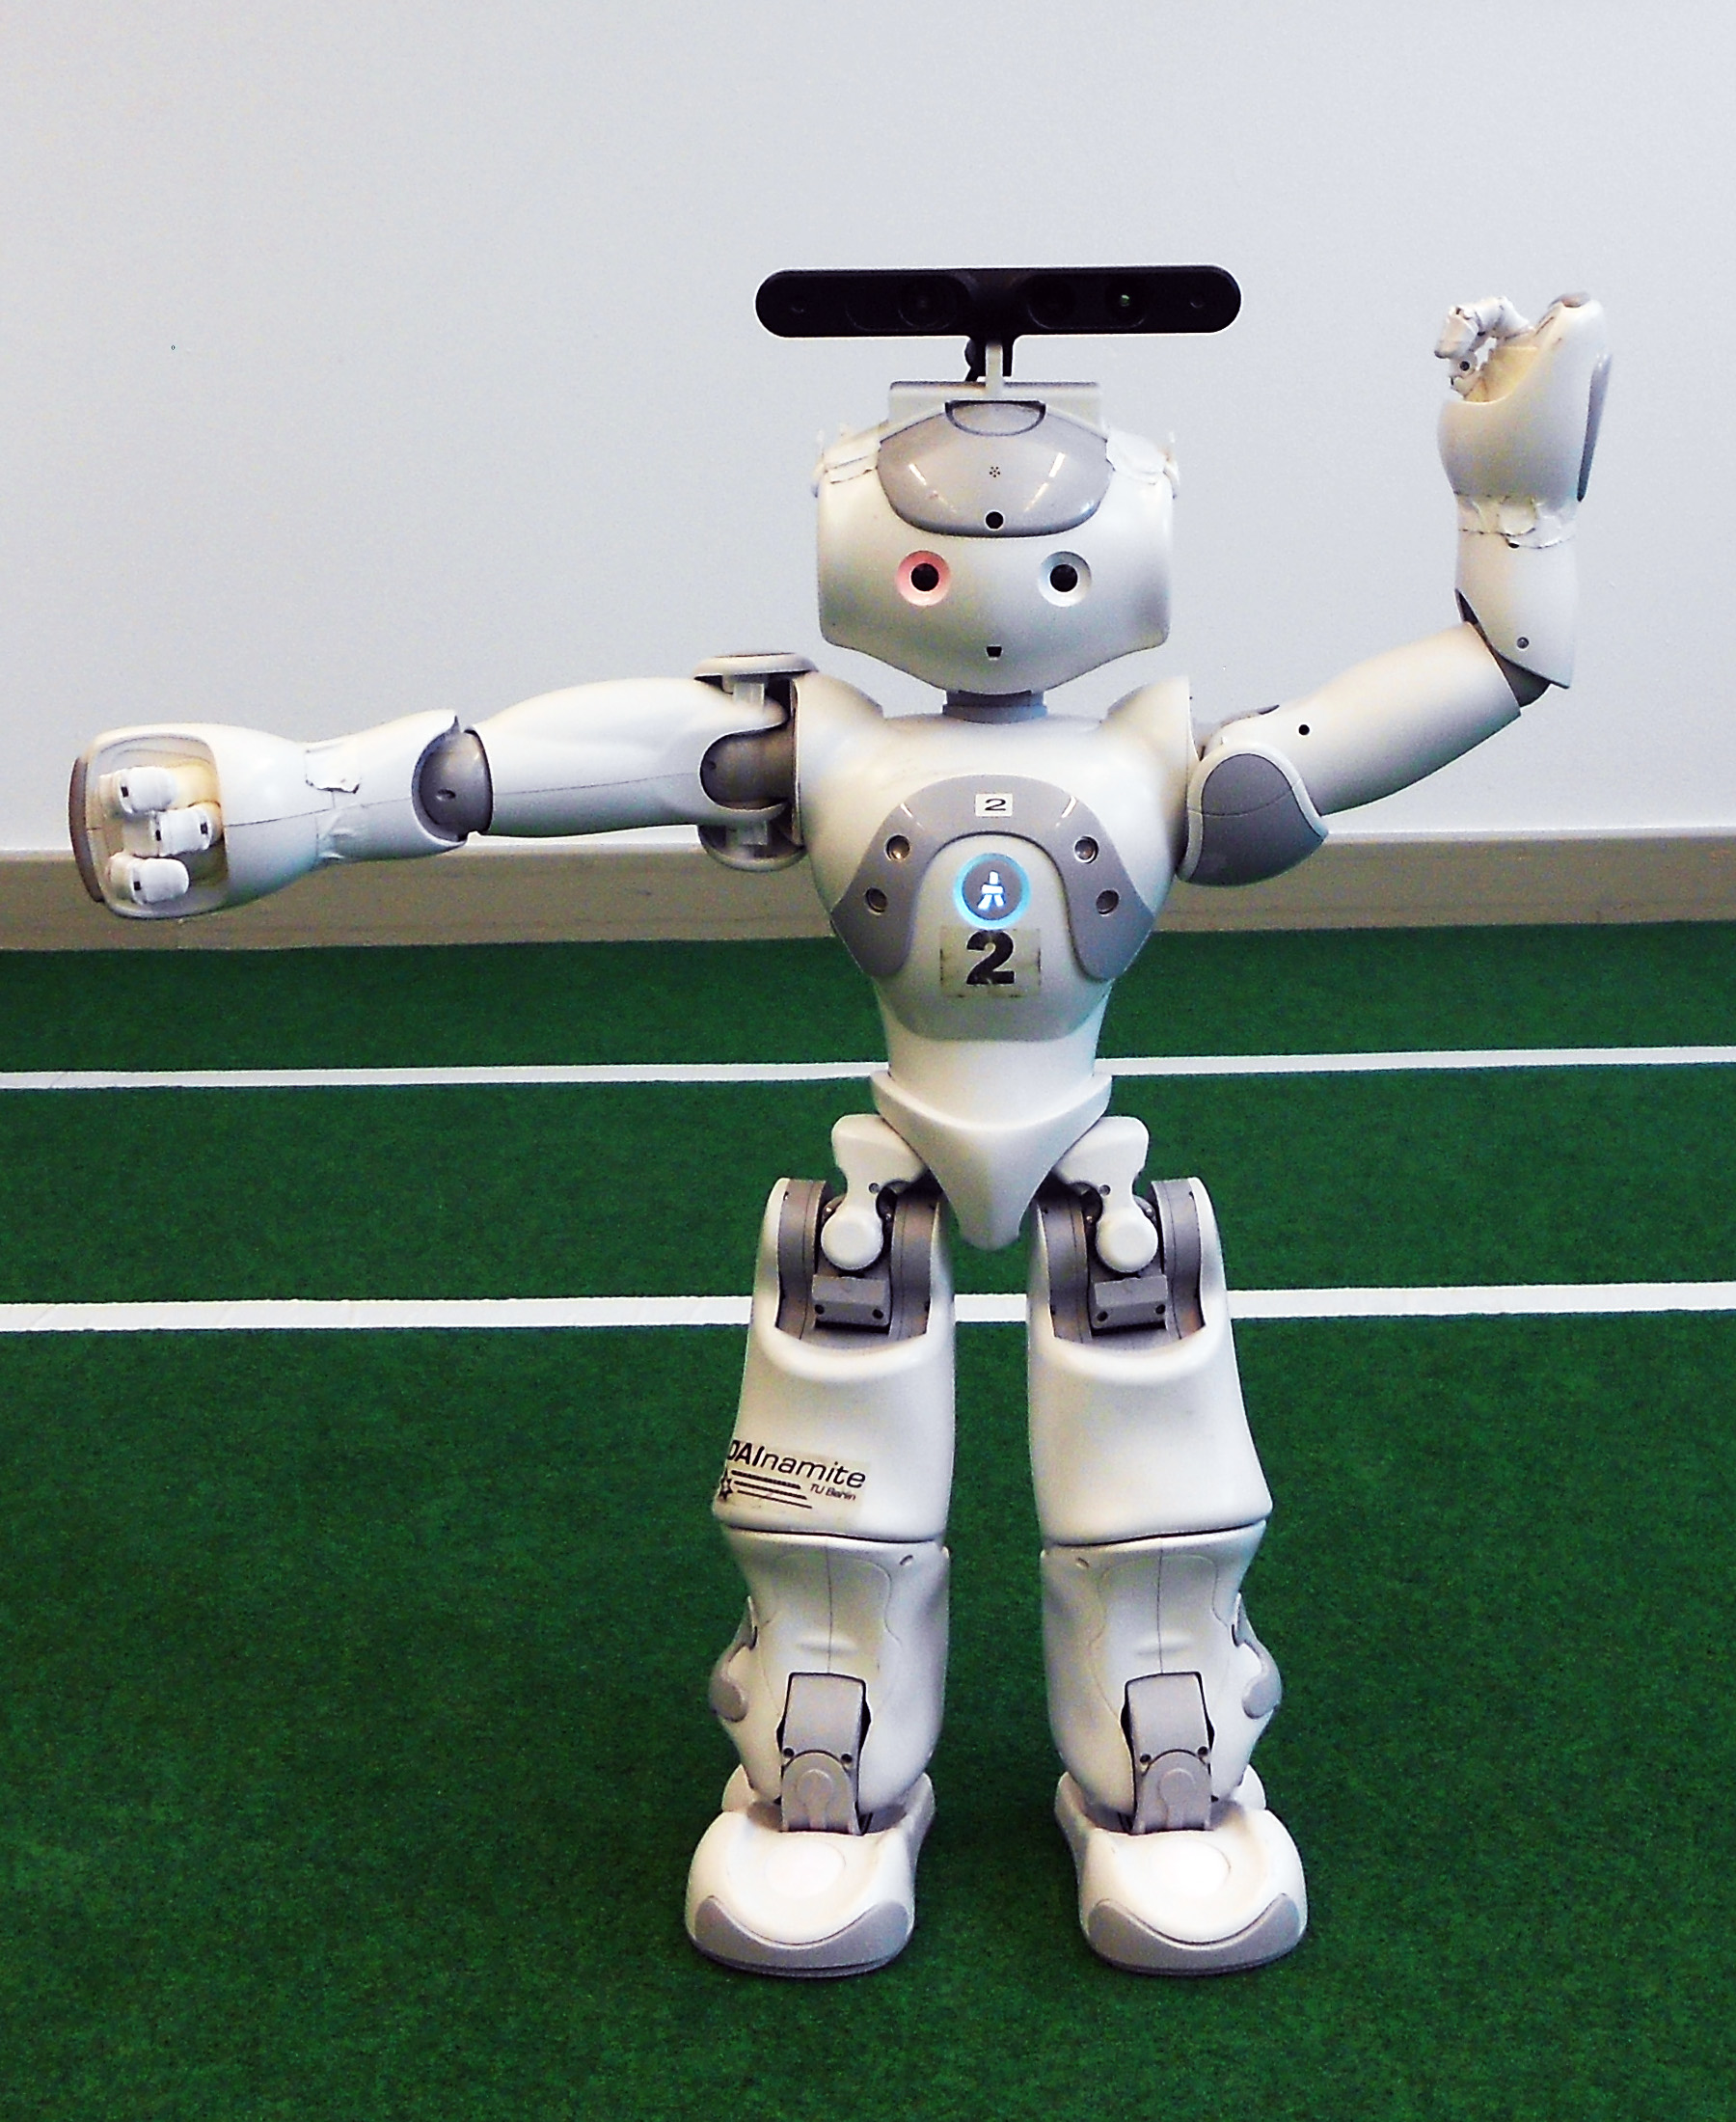
\includegraphics[height=55mm]{figures/result/nao-gg-turn-right.jpg} \caption*{Turn Right } 
	\end{minipage}
	\begin{minipage}
		{.3 
			\textwidth}  
		
		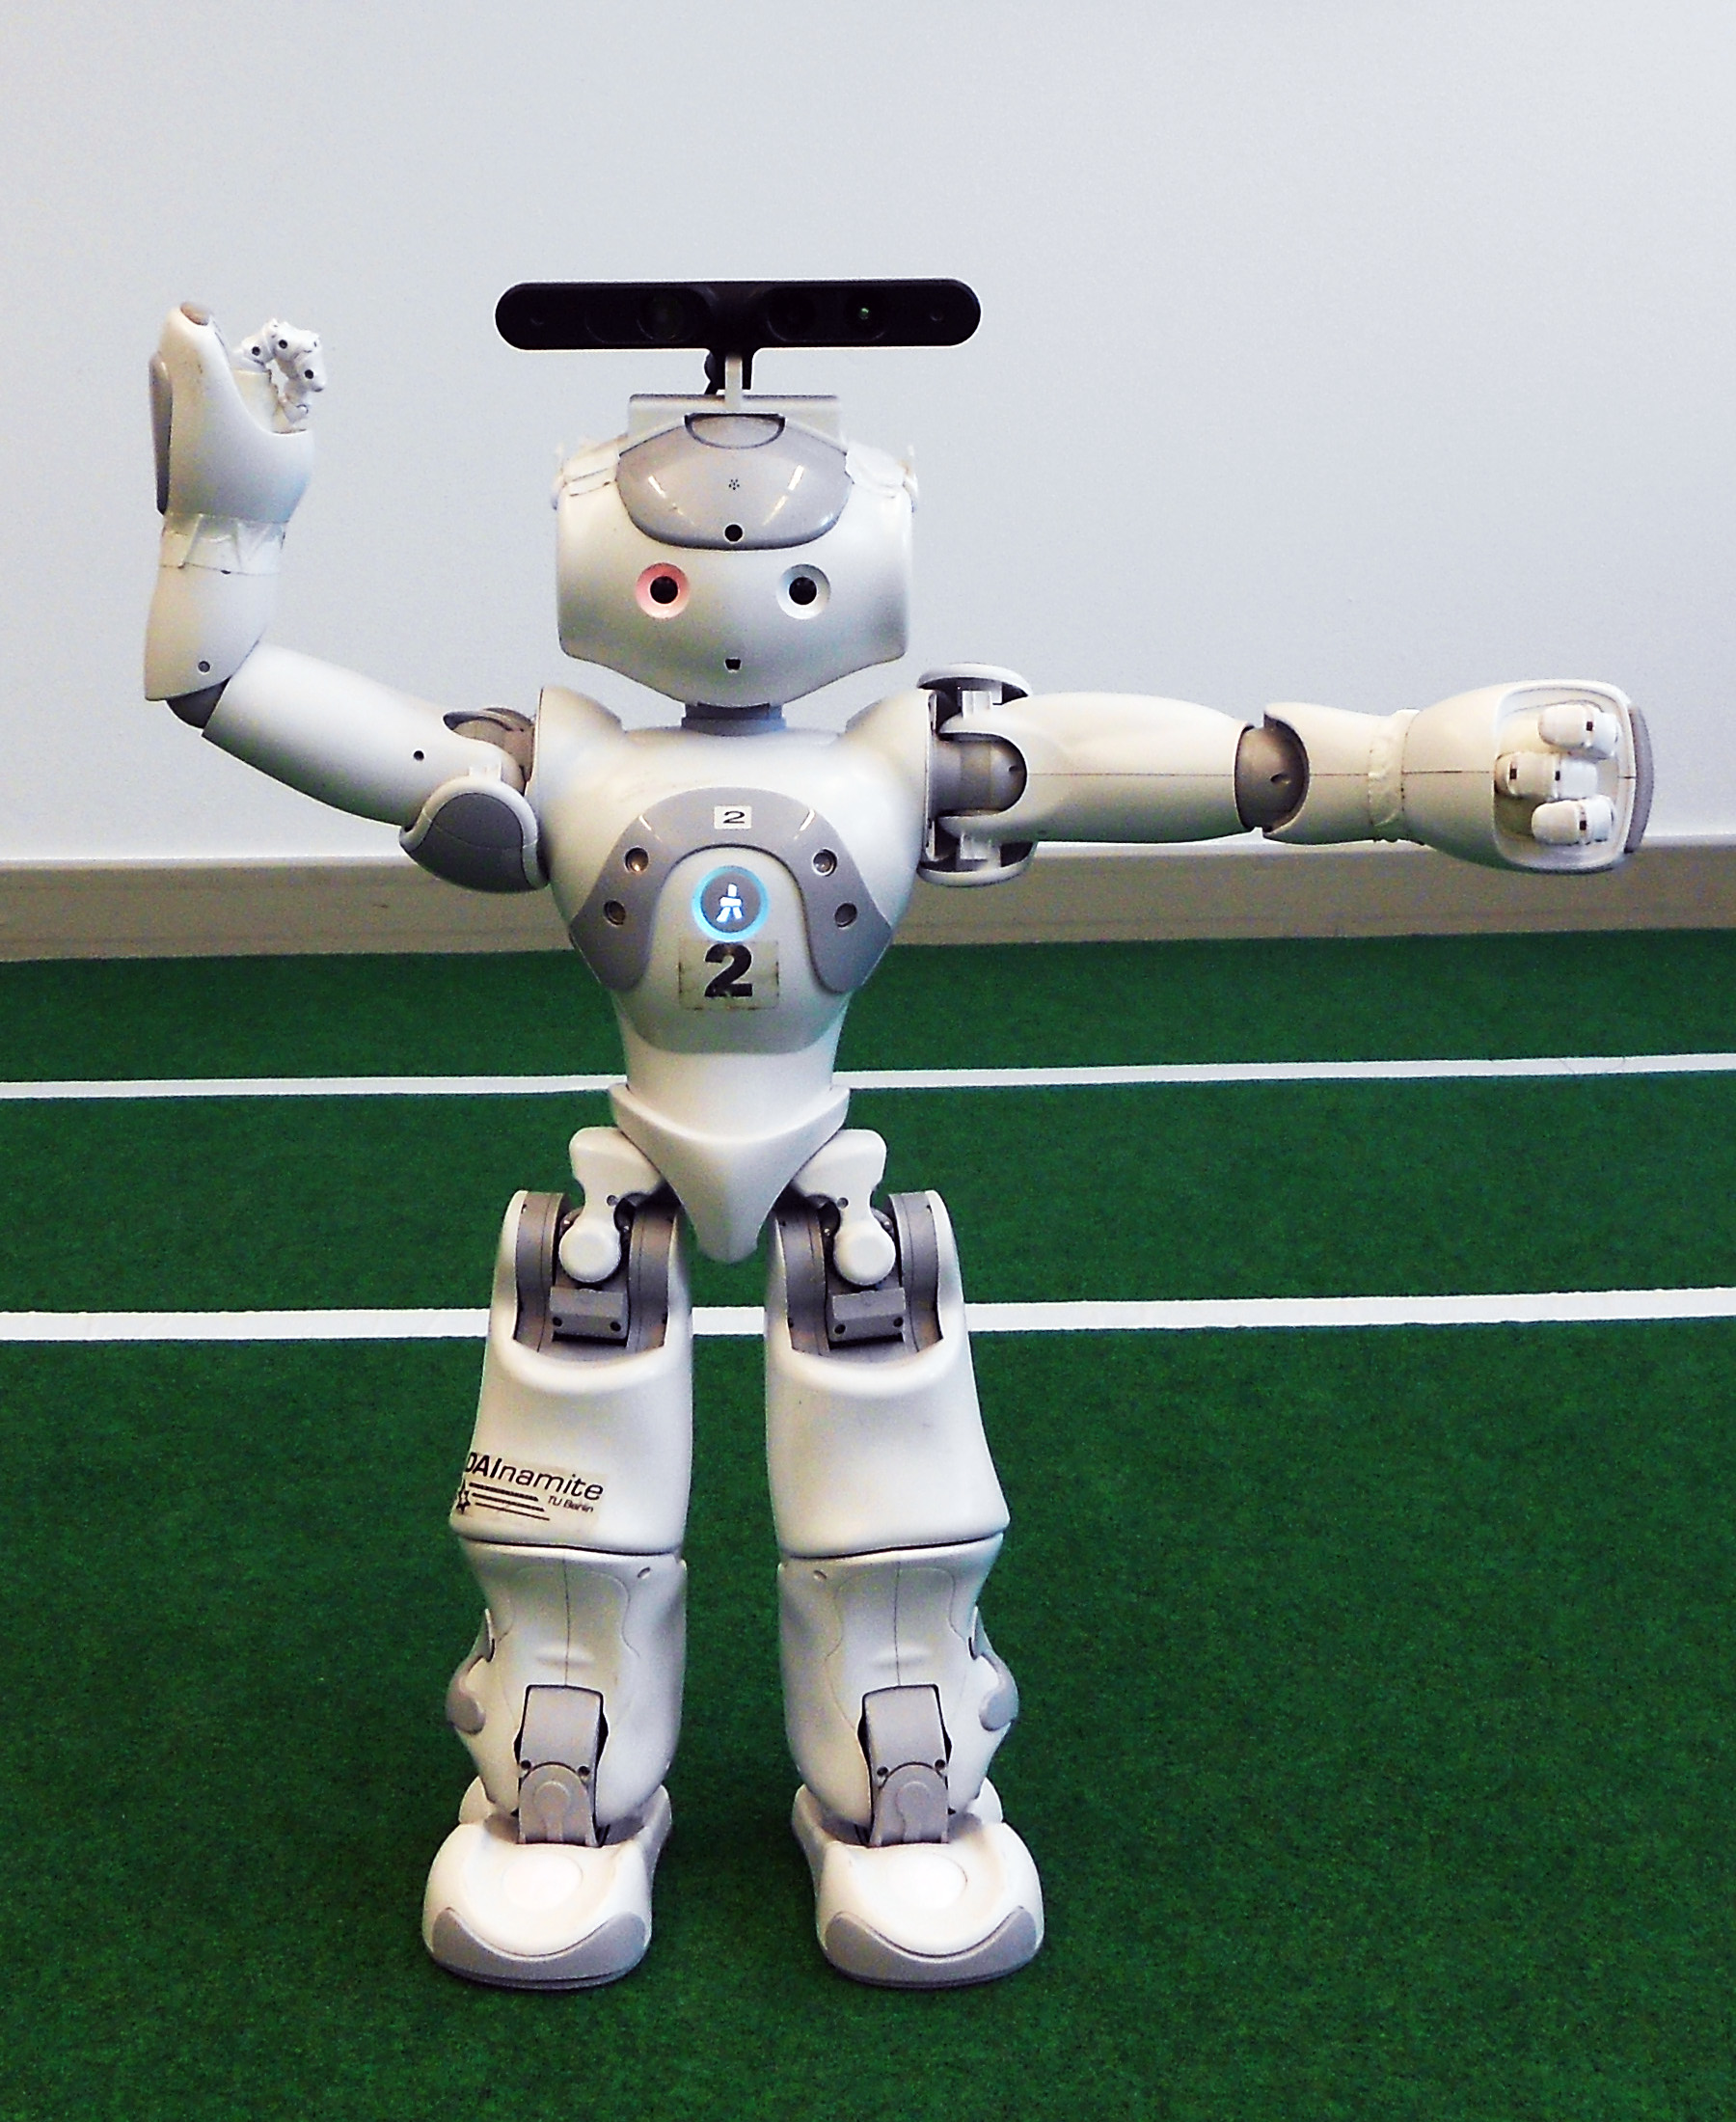
\includegraphics[height=55mm]{figures/result/nao-gg-turn-left.jpg} \caption*{Turn Left }
	\end{minipage}
	\begin{minipage}
		{.3
			\textwidth}  
		
		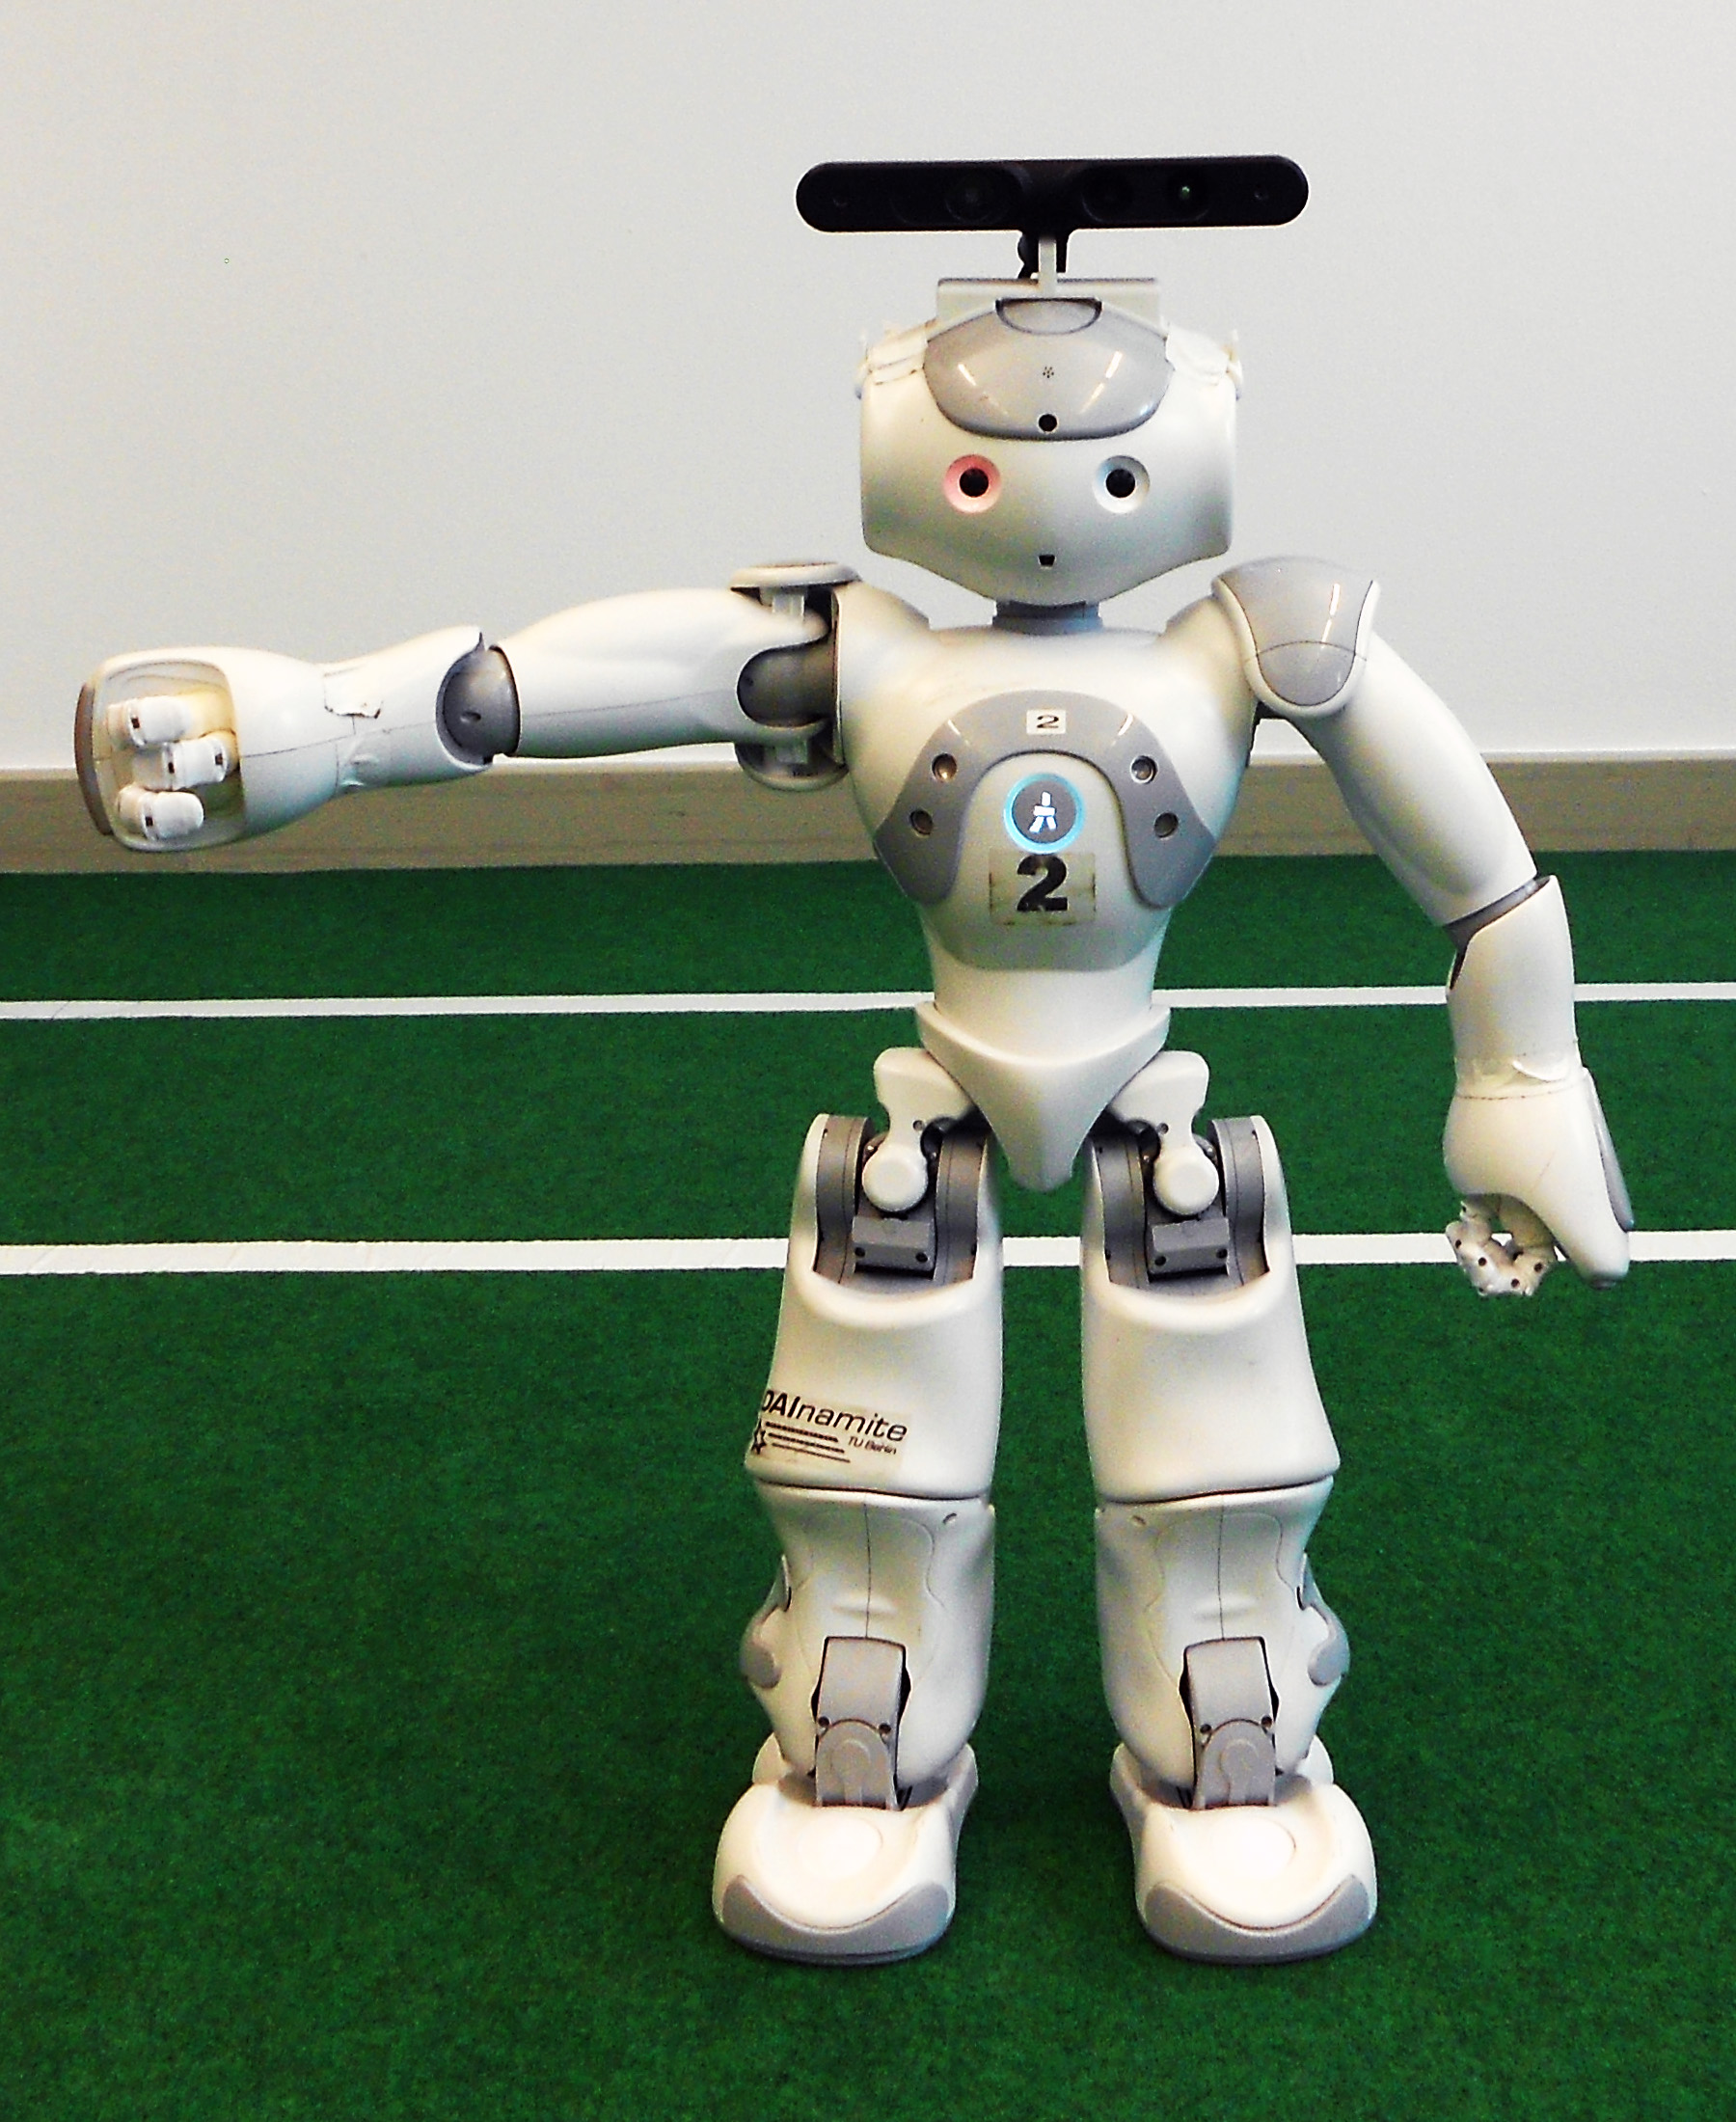
\includegraphics[height=55mm]{figures/result/nao-gg-move-right.jpg} \caption*{Move Right}
	\end{minipage}
	\begin{minipage}
		{.3
			\textwidth}  
		
		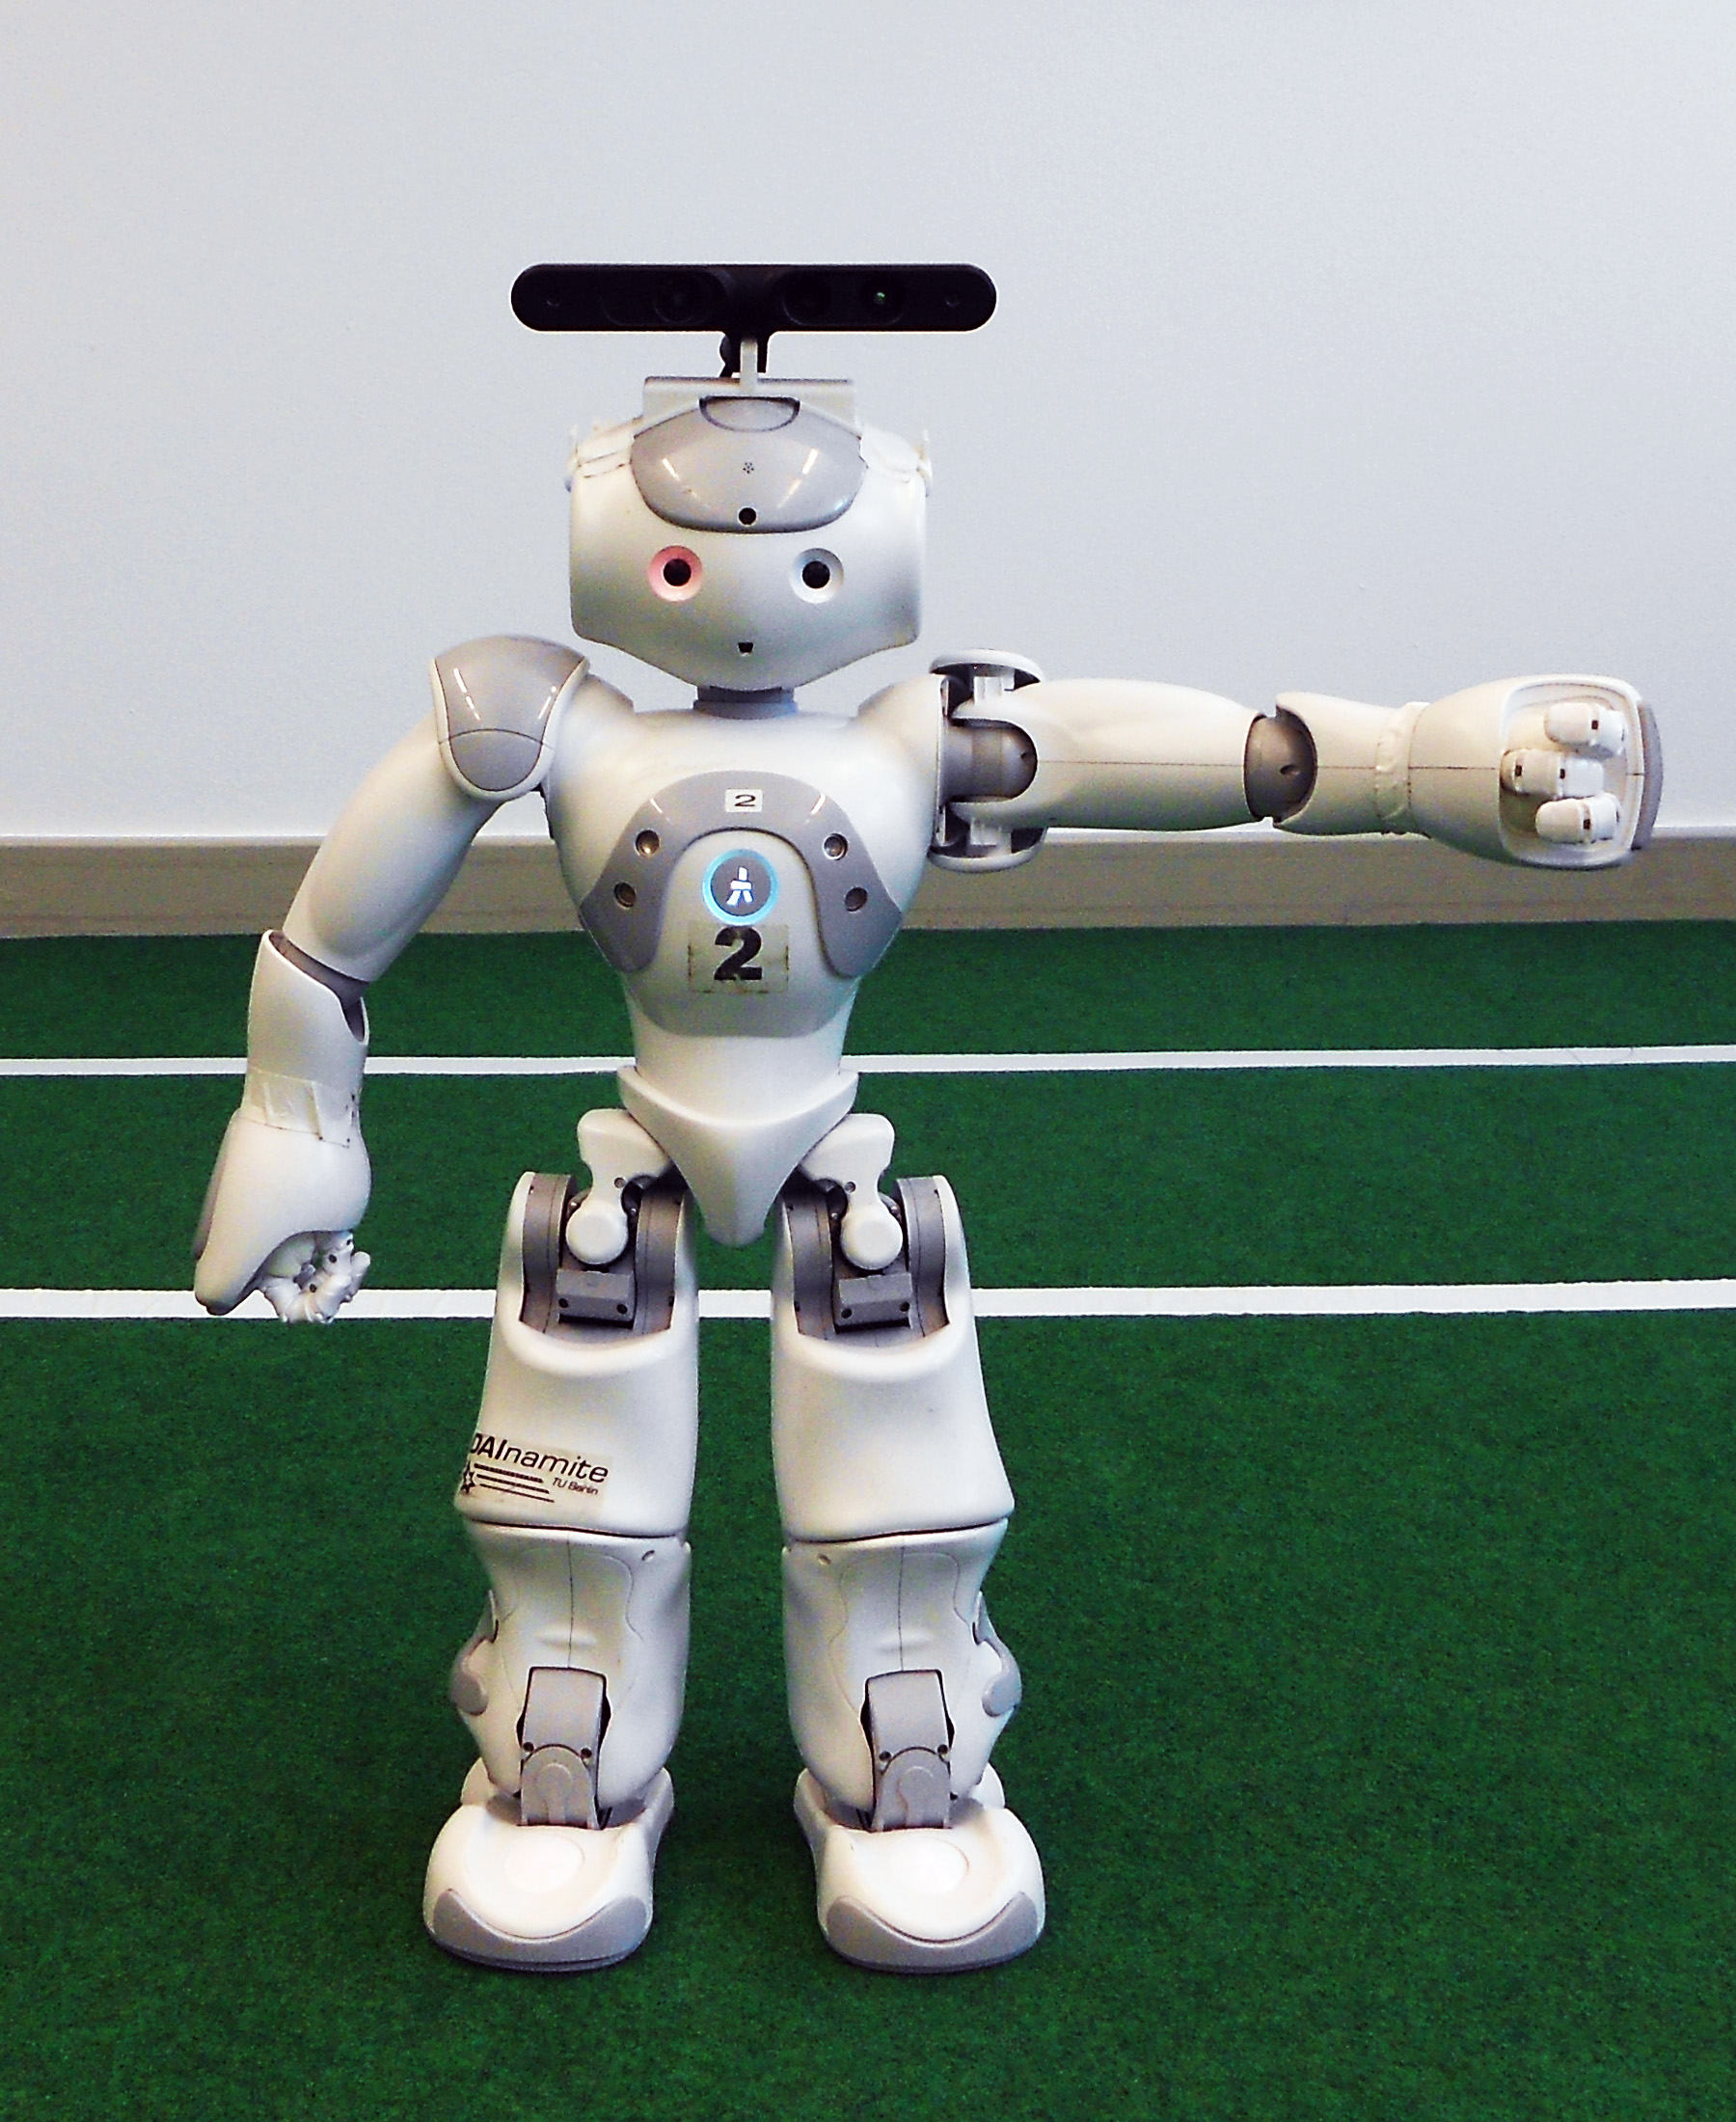
\includegraphics[height=55mm]{figures/result/nao-gg-move-left.jpg} \caption*{Move Left}
	\end{minipage}
	\begin{minipage}
		{.4
			\textwidth}  
		\centering
		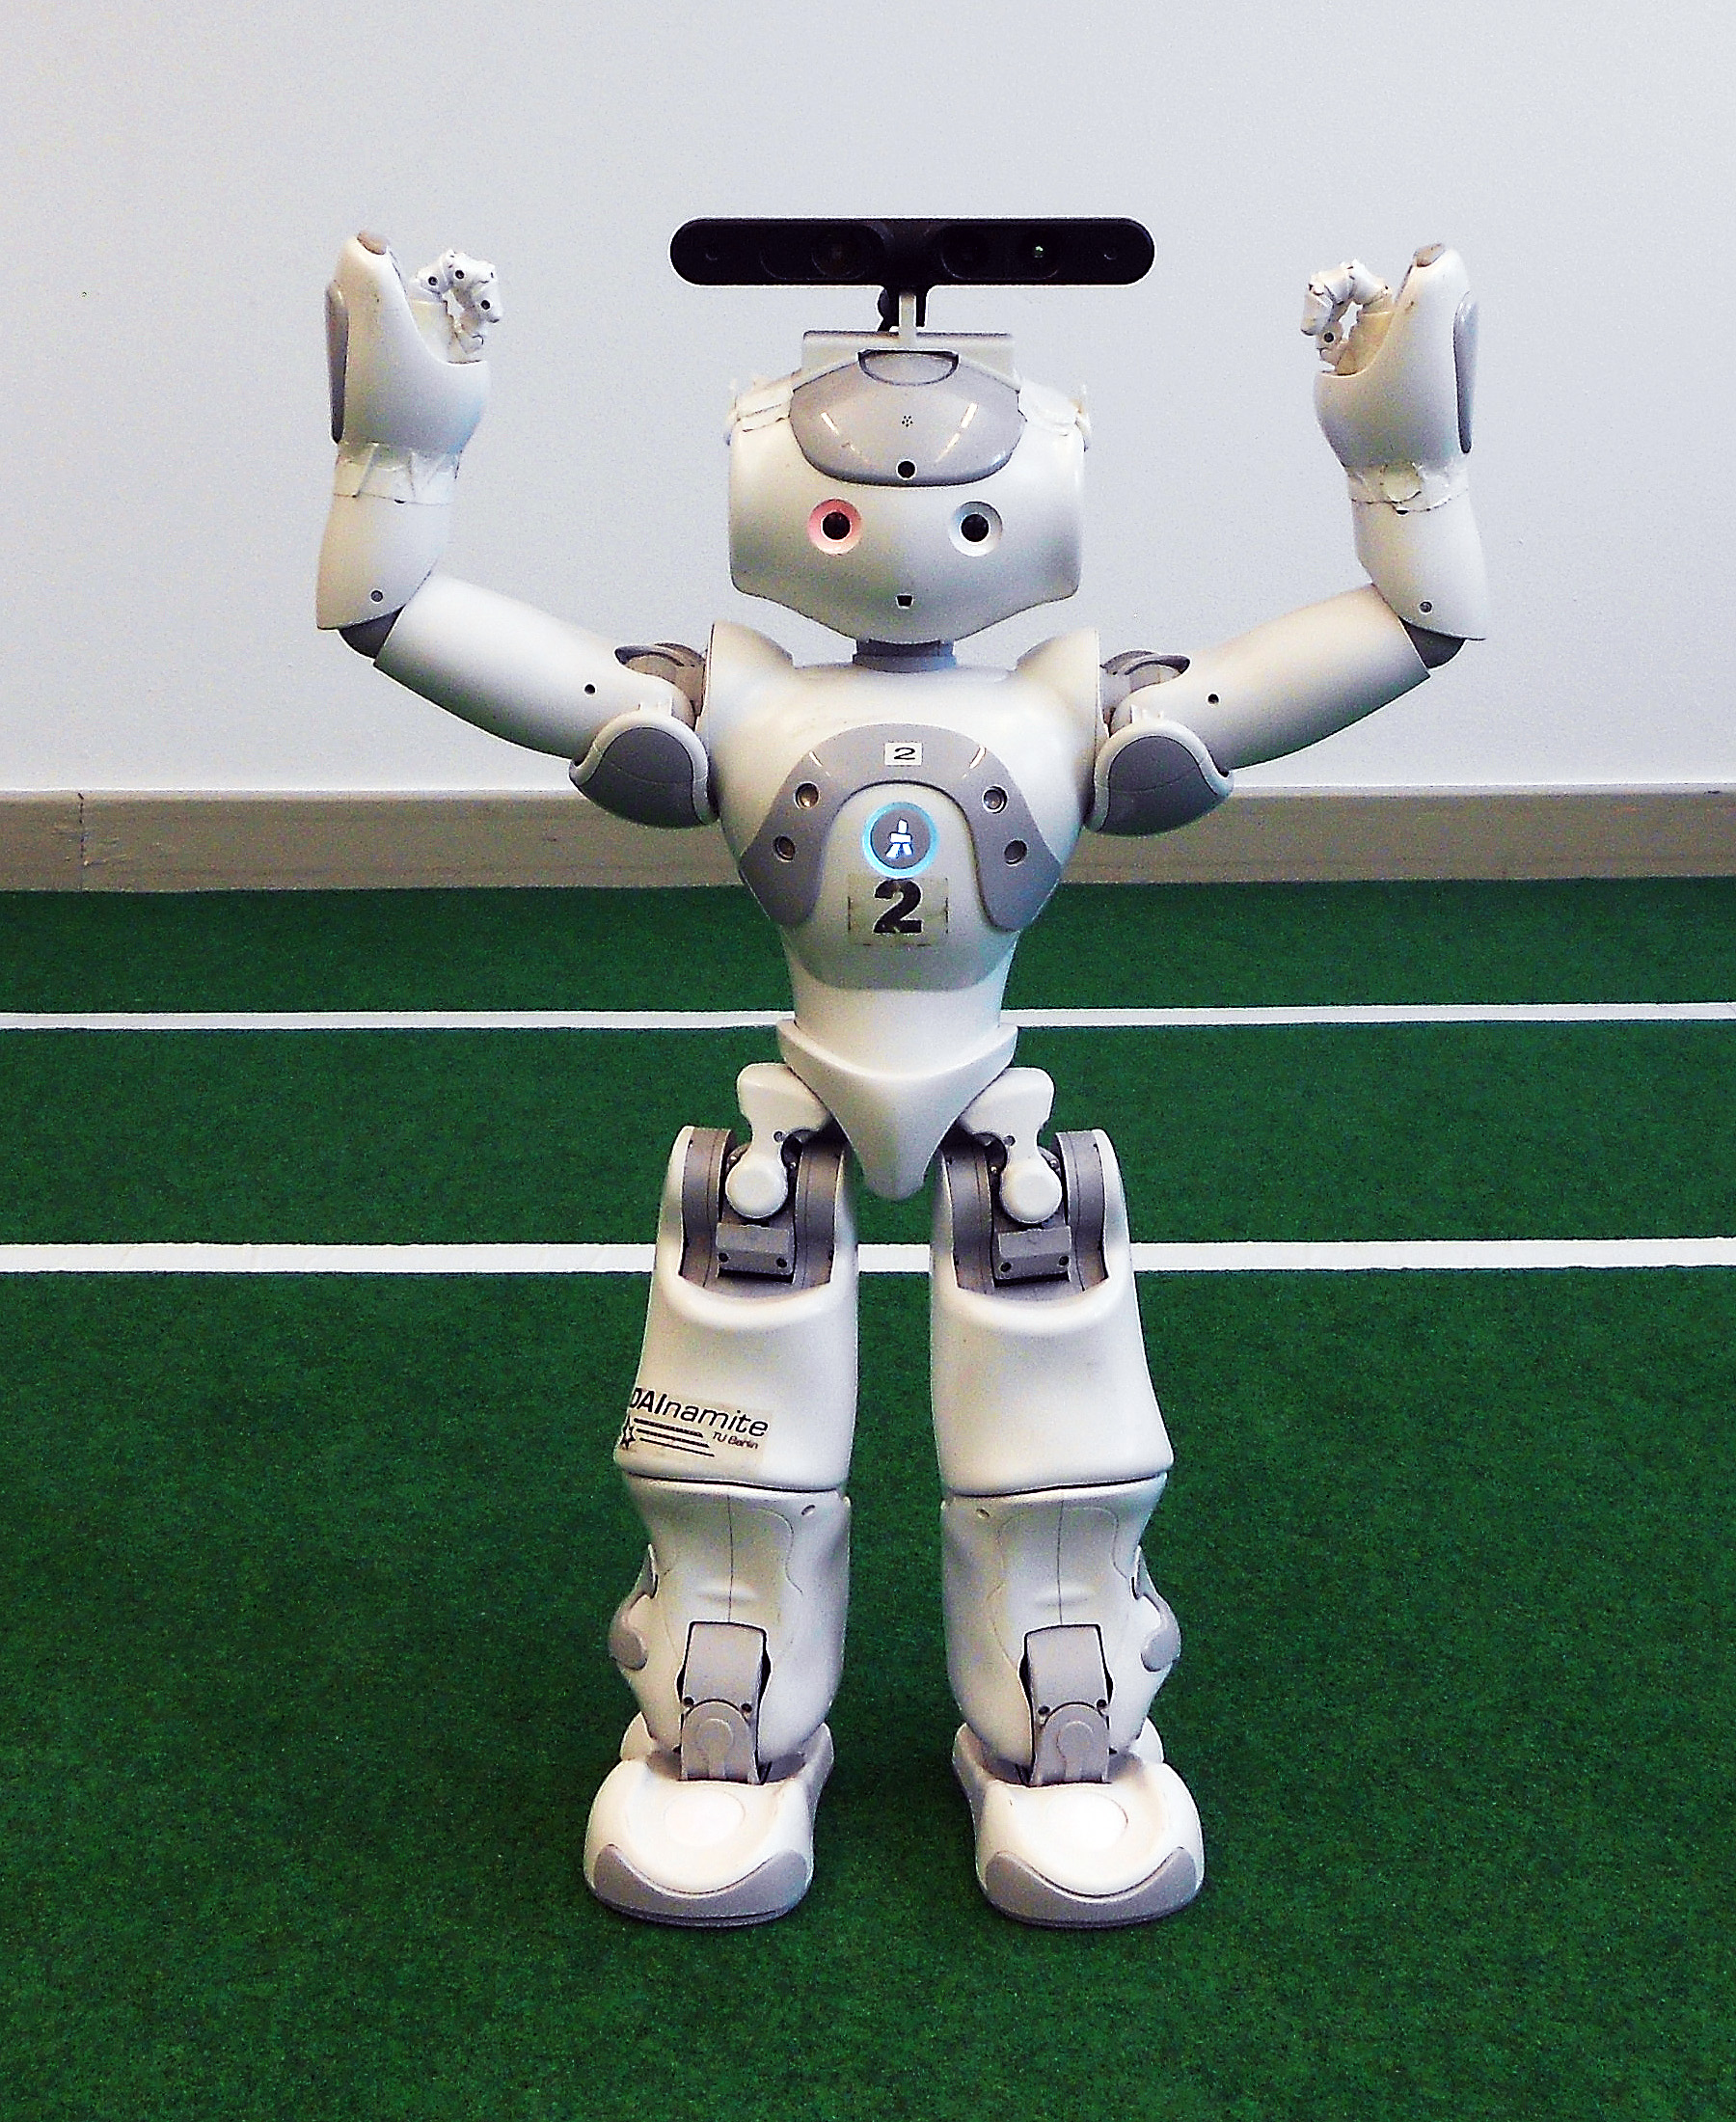
\includegraphics[height=55mm]{figures/result/nao-gg-walk.jpg} 
		\caption*{Walk}
	\end{minipage}	
	\caption{Results of Gesture-To-Gesture translation}
	\label{res:gg}
\end{figure}

